\documentclass{beamer}
\usepackage[utf8]{inputenc}
\usepackage[T1]{fontenc}
\usepackage{lmodern}
\usepackage[ngerman]{babel}
\usepackage{textcomp}
\usepackage{graphicx}
\usepackage{caption3}
\usetheme{CambridgeUS}
\usecolortheme{whale}
\setbeamercolor{frametitle}{fg=subsection in head/foot.bg}
\setbeamercovered{transparent}
\usepackage{epstopdf}

%Die Maße einer Folie in der Beamer-Präsentation betragen 128x96mm%

\title{Diplomarbeit}
\subtitle{Zusammenhang zwischen Makrophytobenthos und Sedimentstruktur in flachen Küstengewässern der deutschen Ostsee}
\author{Antje Kerkow}
\institute[Universität Greifswald]{Studiengang Landschaftsökologie und Naturschutz}
\date{13.5.2014}
\AtBeginSubsection

\begin{document}

\begin{frame}
\titlepage
\end{frame}

\section{Einleitung}
\begin{frame}
\frametitle{Definitionen}
\begin{columns}
\begin{column}{5.5cm}
\begin{figure}
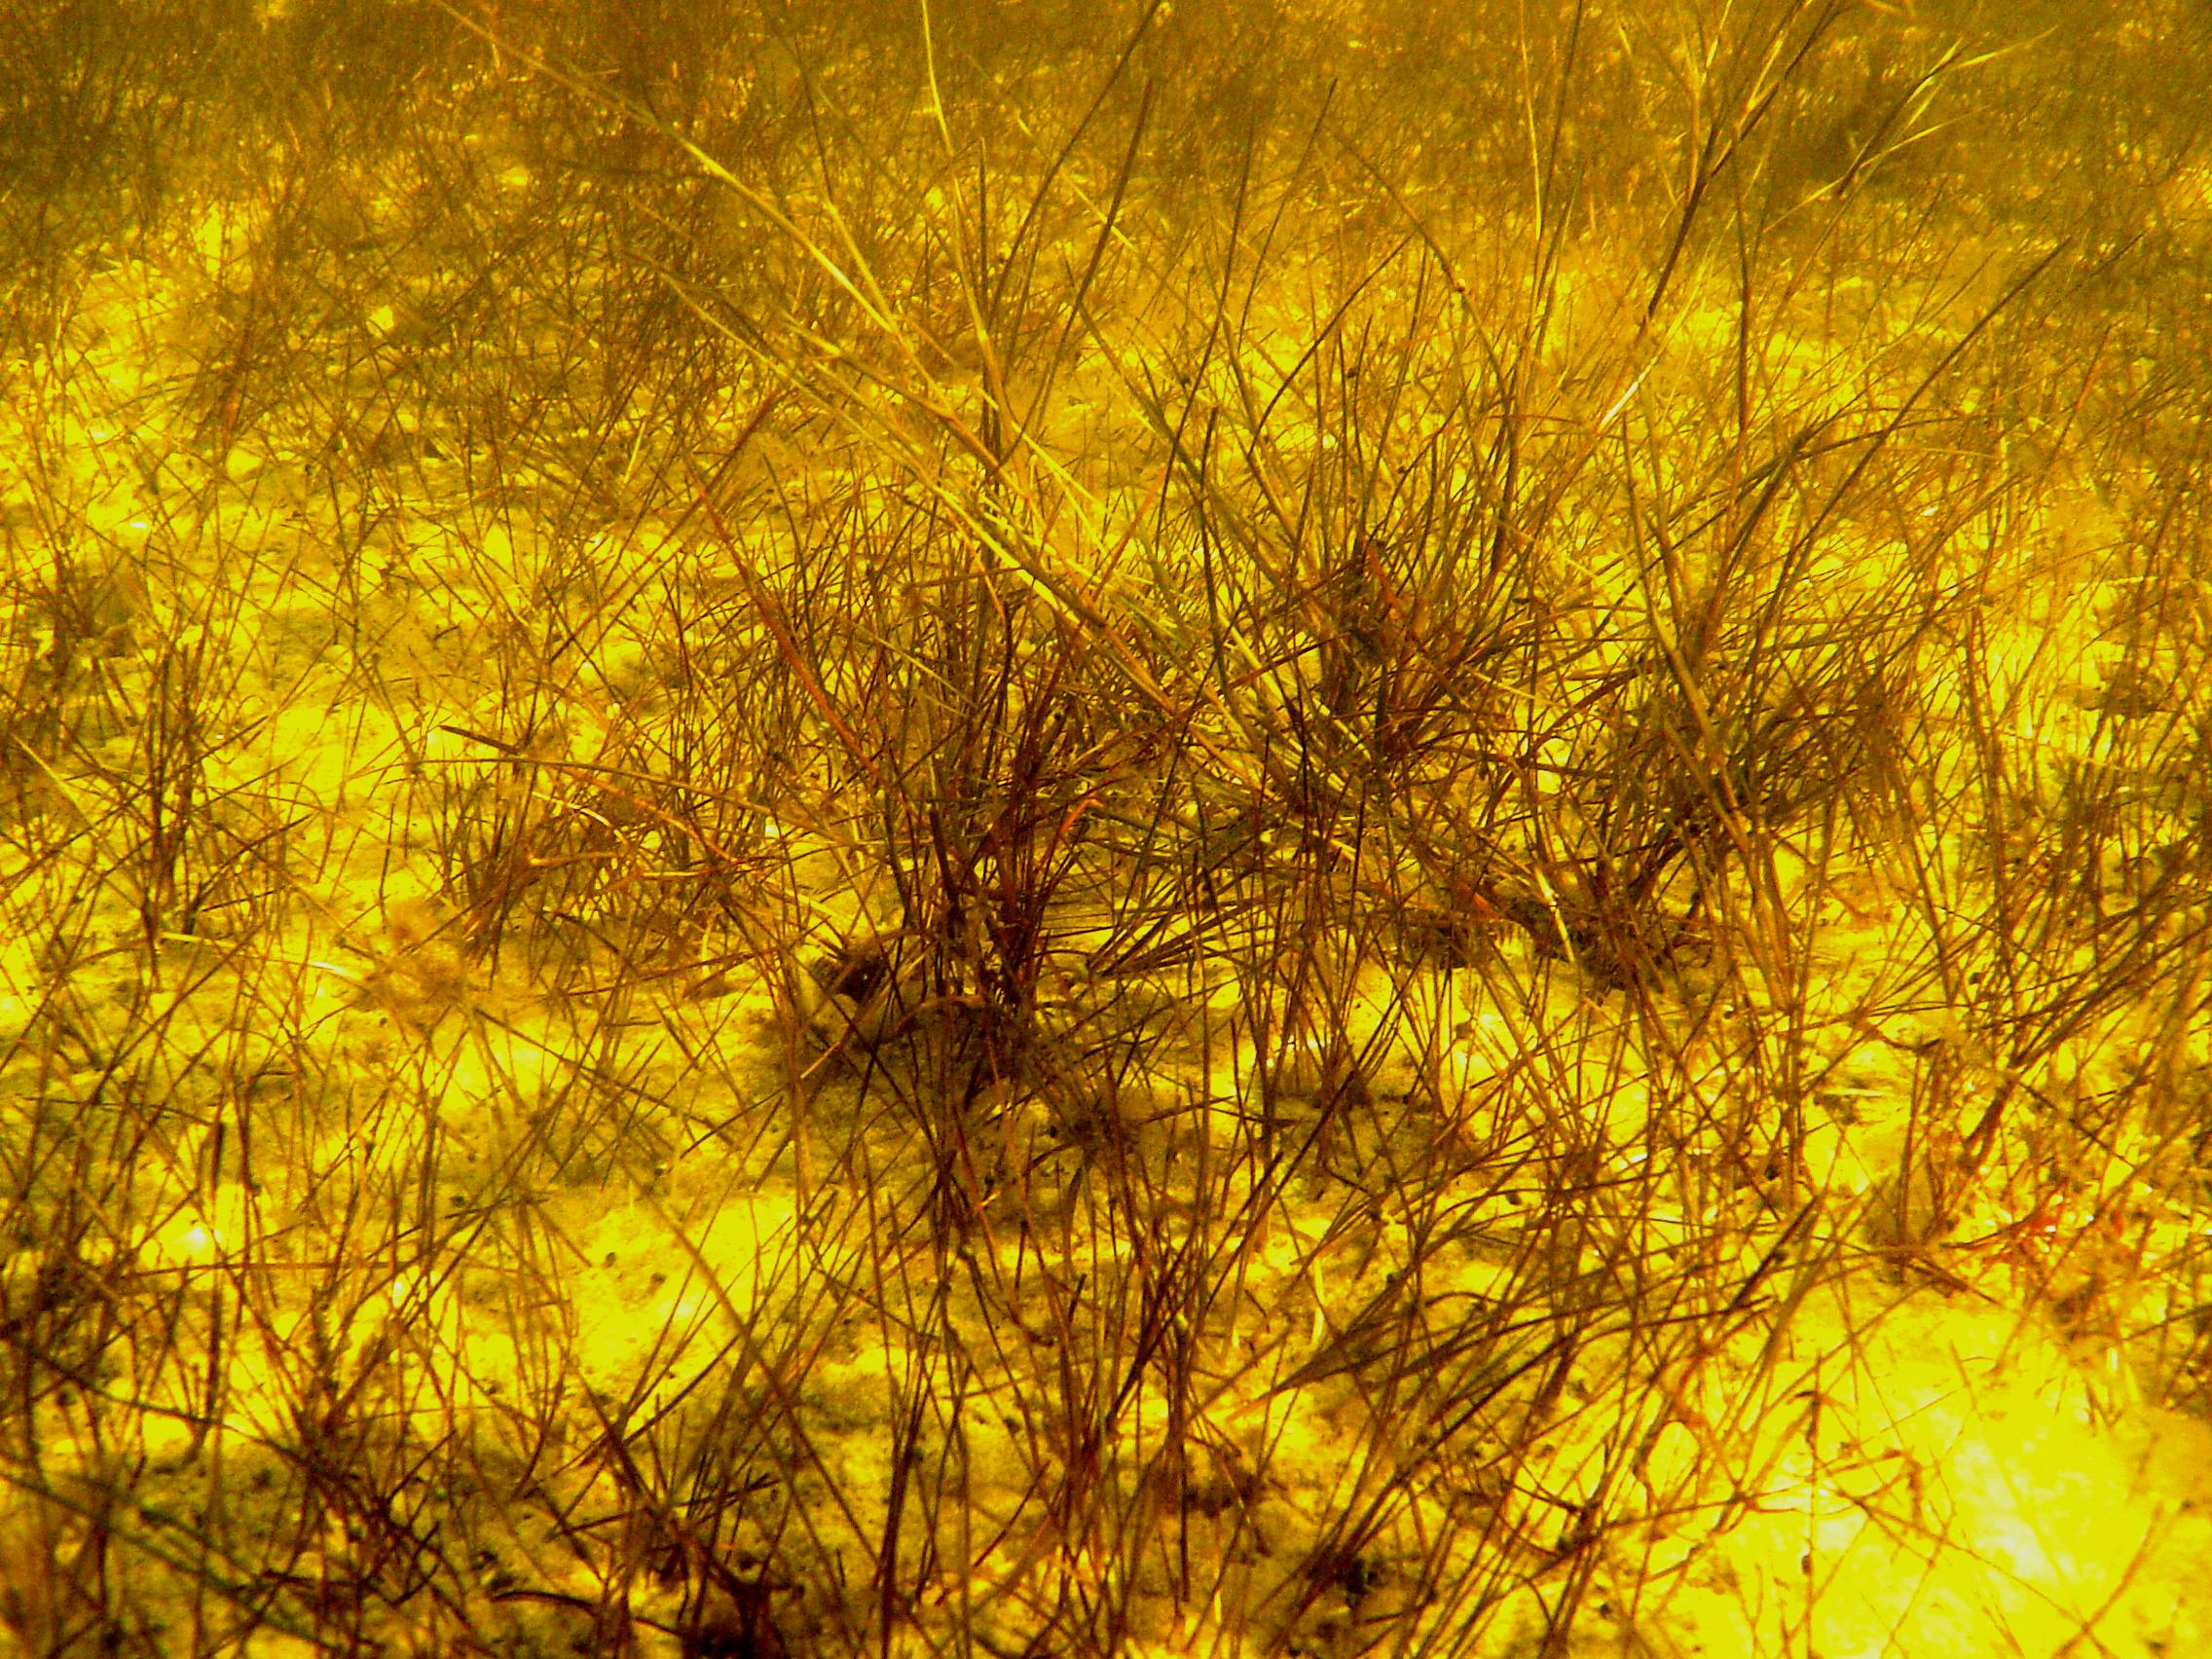
\includegraphics[height=40mm]{images/Fotos/makrophytobenthos.jpg}

Makrophytobenthos
\end{figure}
\end{column}
\begin{column}{5.5cm}
\begin{figure}
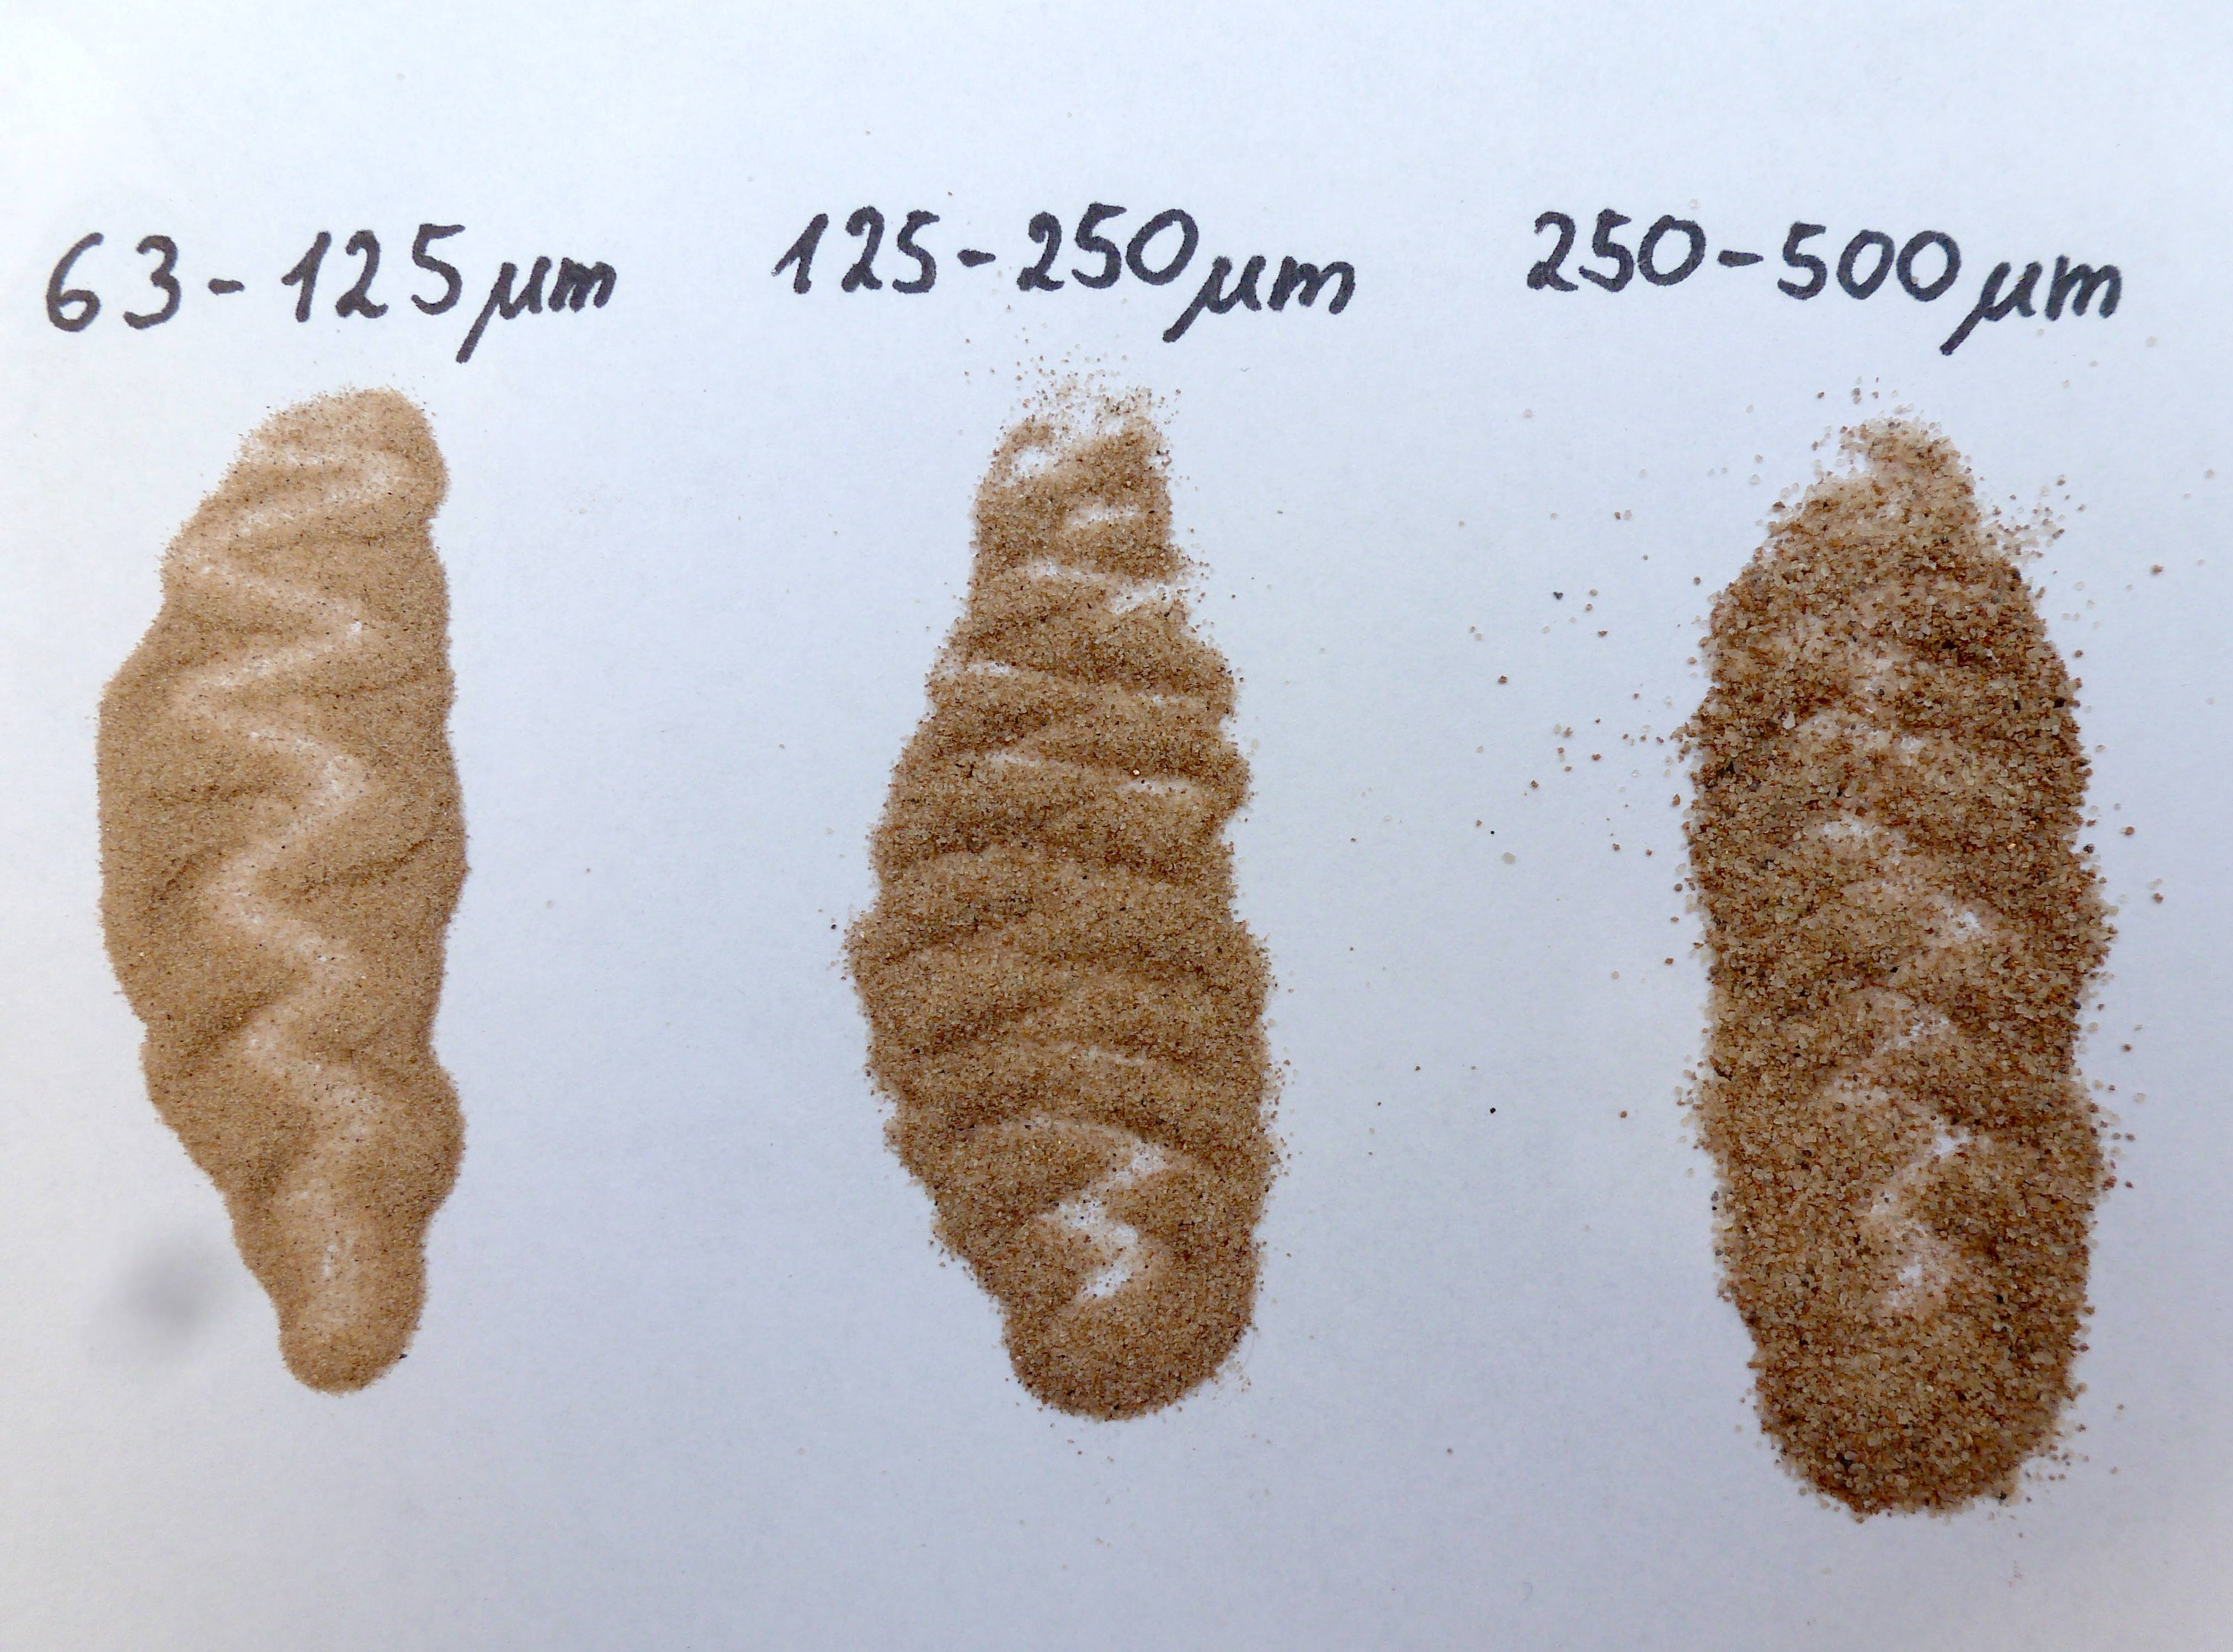
\includegraphics[height=40mm]{images/Fotos/korngroessen.jpg}

Sedimentstruktur
\end{figure}
\end{column}
\end{columns}
\end{frame}

\begin{frame}
\begin{figure}
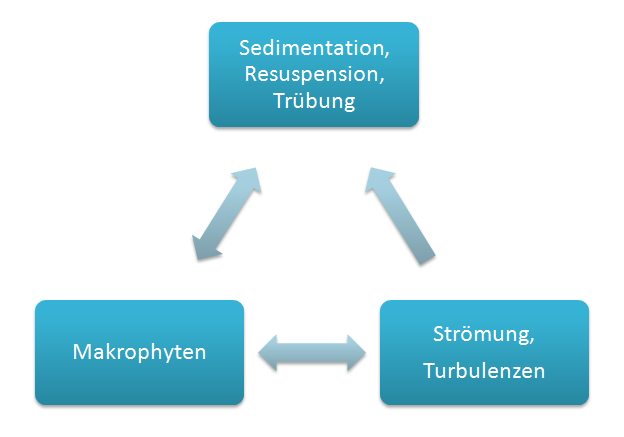
\includegraphics[width=0.7\textwidth]{images/Schema_Pfl_Sedim_Strm}
\end{figure}
\end{frame}

\begin{frame}
\frametitle{Fragestellungen dieser Arbeit}
\begin{enumerate}
\pause
\item Ist in dichten Makrophytenbeständen das Sediment feiner?
\pause
\item Korreliert der Anteil der Pflanzen in der Wassersäule mit der mittleren Korngröße?
\pause
\item Ist der organische Gehalt der Sedimente höher?
\pause
\item Verändern sich Artenzusammensetzung und Vegetationsstruktur im Jahresverlauf?
\pause
\item Verändert sich die mittlere Korngröße und der organische Gehalt der Sedimente im Jahresverlauf? 
\end{enumerate}
\end{frame}

\section{Untersuchungsgebiete}
%\subsection{Alle Stationen entlang des Salzgradienten}
%\begin{frame}
%\frametitle{Alle Stationen entlang des Salzgradienten}
%\begin{figure}
%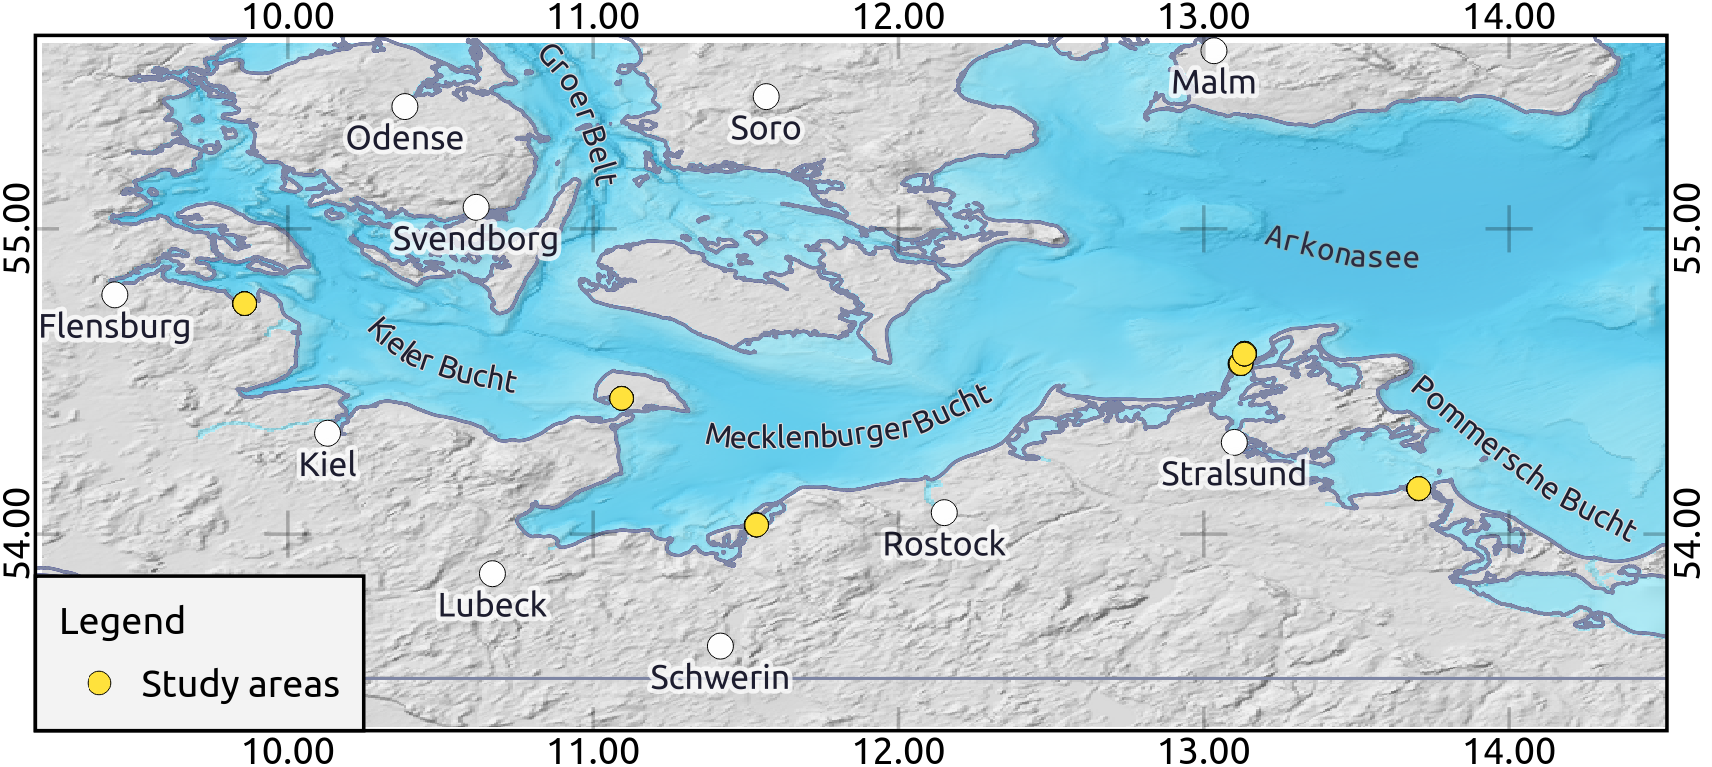
\includegraphics[scale=0.24]{images/Uebersicht.png}
%\end{figure}
%\begin{center}
%Geltinger B., Orther B., Salzhaff, Hiddenseer B., Spandowerh.Wiek
%\end{center}
%\end{frame}

\subsection{Hiddenseer Standorte}

\begin{frame}
\frametitle{Untersuchungsgebiet}
\begin{figure}
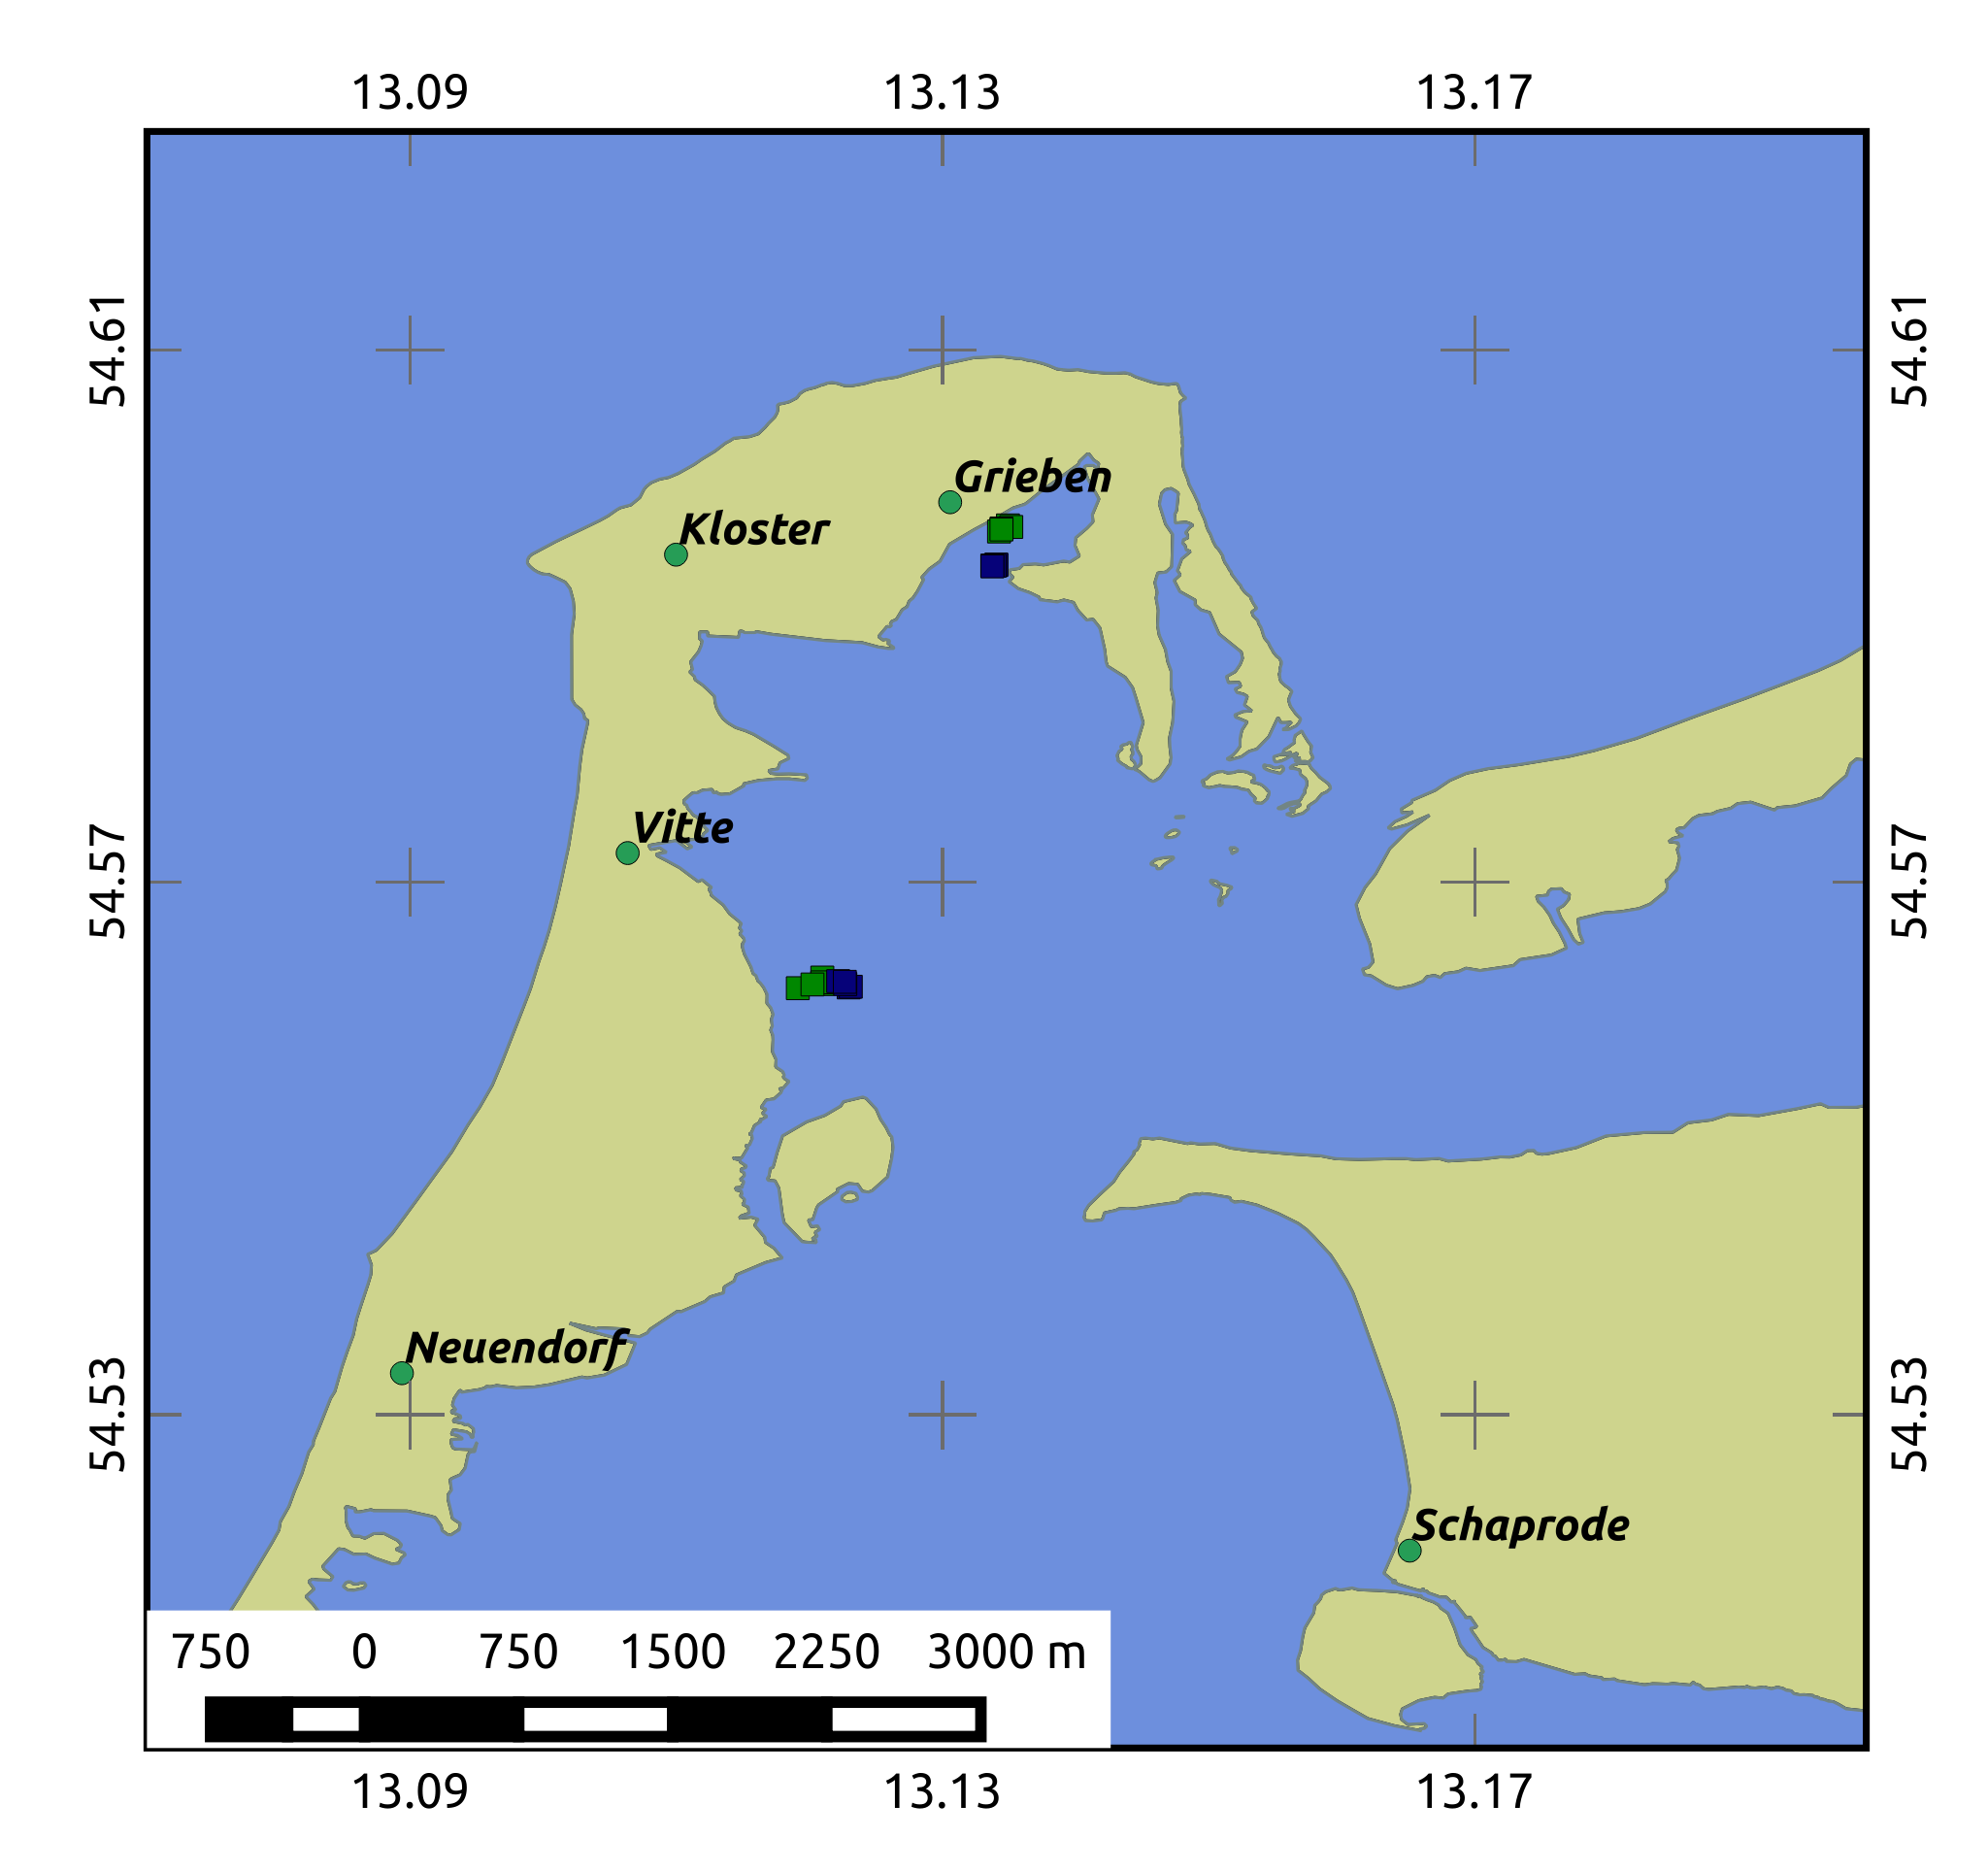
\includegraphics[height=0.8\textheight]{images/Hiddensee.png}
\end{figure}
\end{frame}

\begin{frame}
\frametitle{Vitte}
\begin{figure}
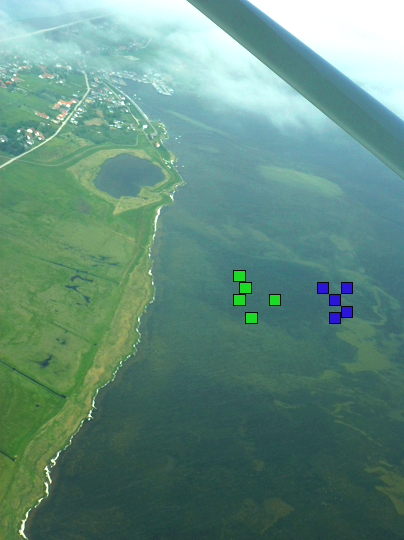
\includegraphics[height=0.8\textheight]{images/Fotos/vitte.png}
\end{figure}
\end{frame}

\begin{frame}
\frametitle{Grieben}
\begin{figure}
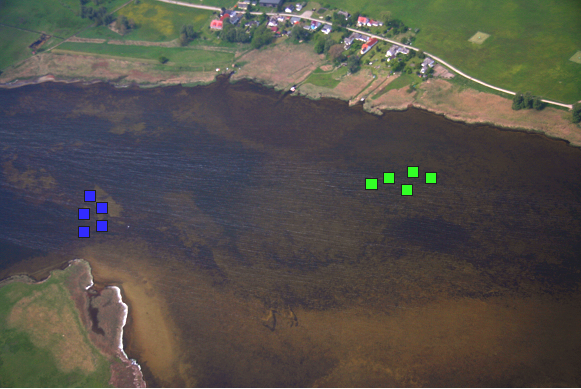
\includegraphics[width=0.8\textwidth]{images/Fotos/griebenerbucht.png}
\end{figure}
\end{frame}

\section{Methoden}
\subsection{Vegetation}

\begin{frame}
\frametitle{Vegetationskartierung}
\begin{columns}
\begin{column}{5.5cm}
\begin{figure}
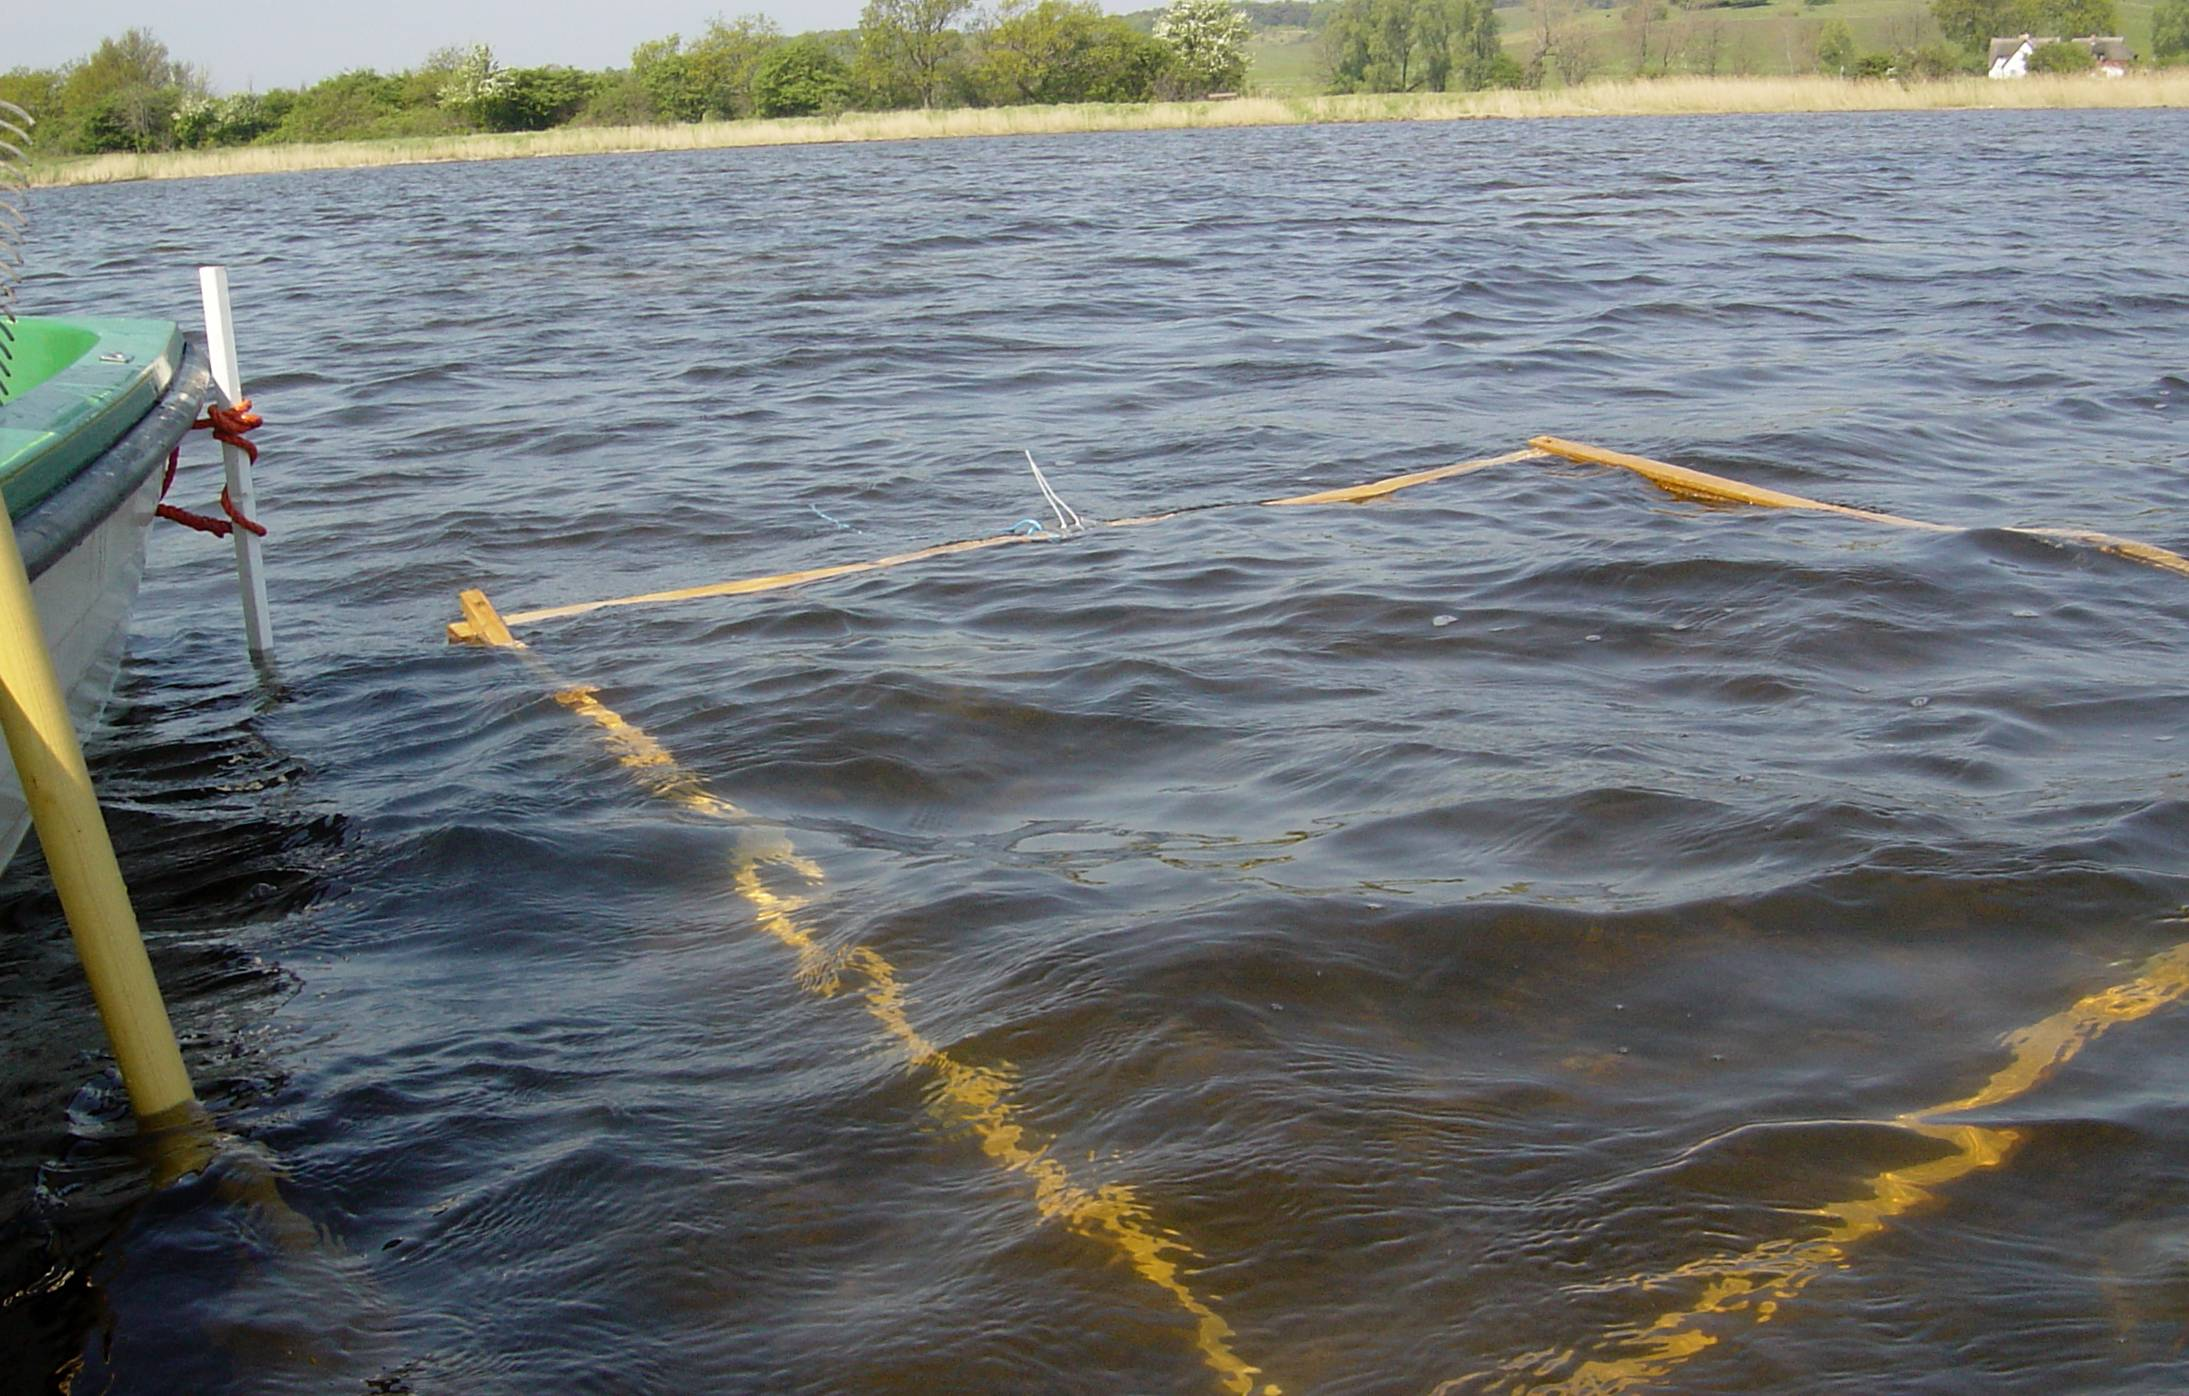
\includegraphics[height=35mm]{images/Fotos/vegetationsrahmen.jpg}
\end{figure}
\end{column}
\begin{column}{5.5cm}
\begin{figure}
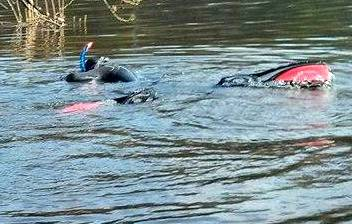
\includegraphics[height=35mm]{images/Fotos/schnorchelnklein2.jpg}
\vspace*{+5mm}
\end{figure}
\end{column}
\end{columns}
\end{frame}


\begin{frame}
\begin{columns}
\begin{column}{5.5cm}
\begin{block}{Absolute Deckung}
Deckungsgrade: 
1\%; 1-4\%; 5\%; 10\%; 20\%; ... ; 100\% 
\end{block}
\begin{figure}
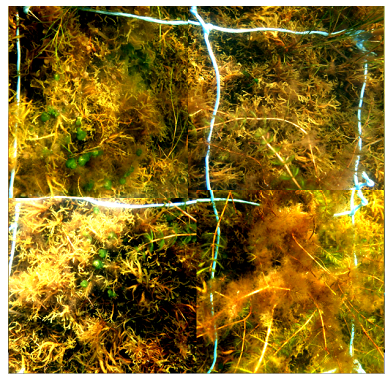
\includegraphics[height=40mm]{images/plotpictures/V+M.png}
\end{figure}
\end{column}
\visible<2>{
\begin{column}{5.5cm}
\begin{block}{Höhenstufenkartierung}
Höhenstufen: 
5cm; 10cm; 20cm; 30cm; 40cm ...
\end{block}
\begin{figure}
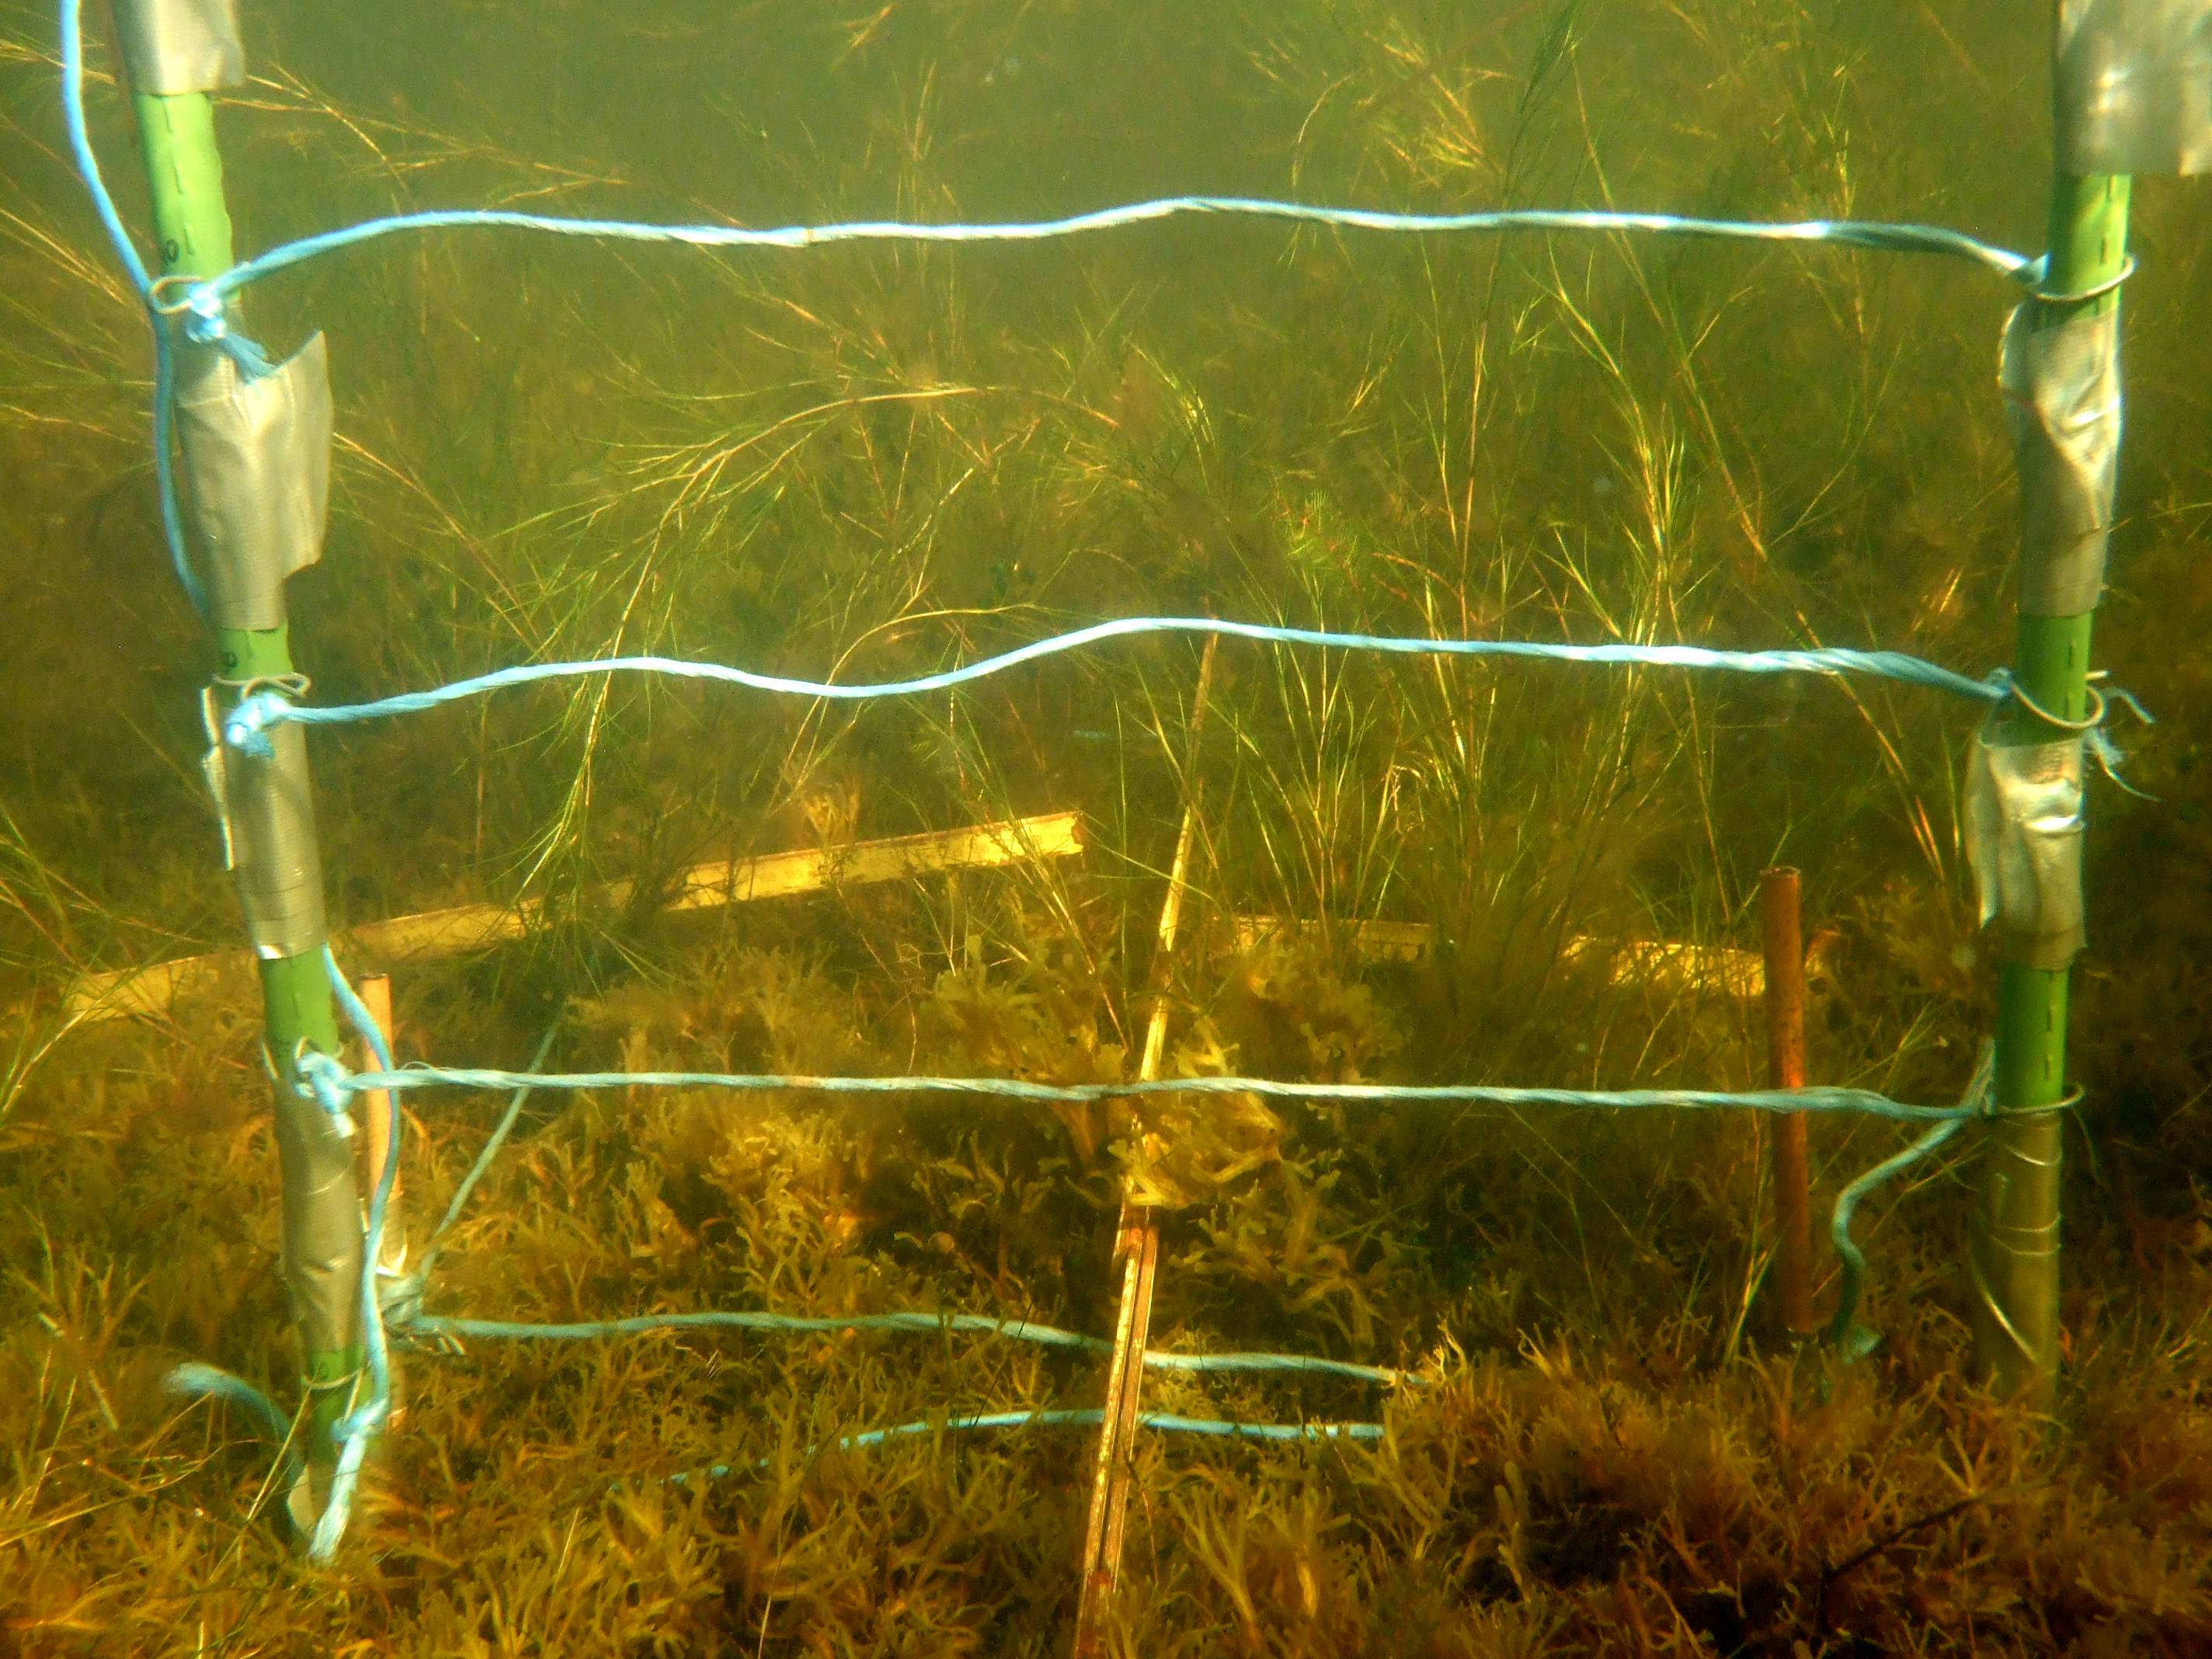
\includegraphics[height=40mm]{images/Fotos/DSCF0510.JPG}
\end{figure}
\end{column}}
\end{columns}
\end{frame}

\begin{frame}
\frametitle{PVI-Berechnung}
\begin{block}{Traditionell:}
\begin{equation*}
\frac{\text{Mittlere Wuchshöhe} * \text{Deckung}}{\text{Wassertiefe}}
\end{equation*}
\end{block}
\pause
\begin{block}{Verändert:}
\begin{align*}
 PVI &=\frac{\sum_{i=a}^n \frac{H_i * C_i}{100}}{\text{mittlere Wassertiefe}} & H_i &=\text{Länge einer jeden Höhenschicht}\\ 
 & & C_i &=\text{Deckung auf dieser Höhenschicht}\\
 & & a-n &=\text{Höhenstufen vom Boden}\\
 & &     &\text{\quad bis zur Wasseroberfläche}\\
\end{align*}
\end{block}
\end{frame}

\subsection{Sediment}
\begin{frame}
\frametitle{Sediment-Probenahme}
\begin{columns}
\begin{column}{6.4cm}
\begin{figure}
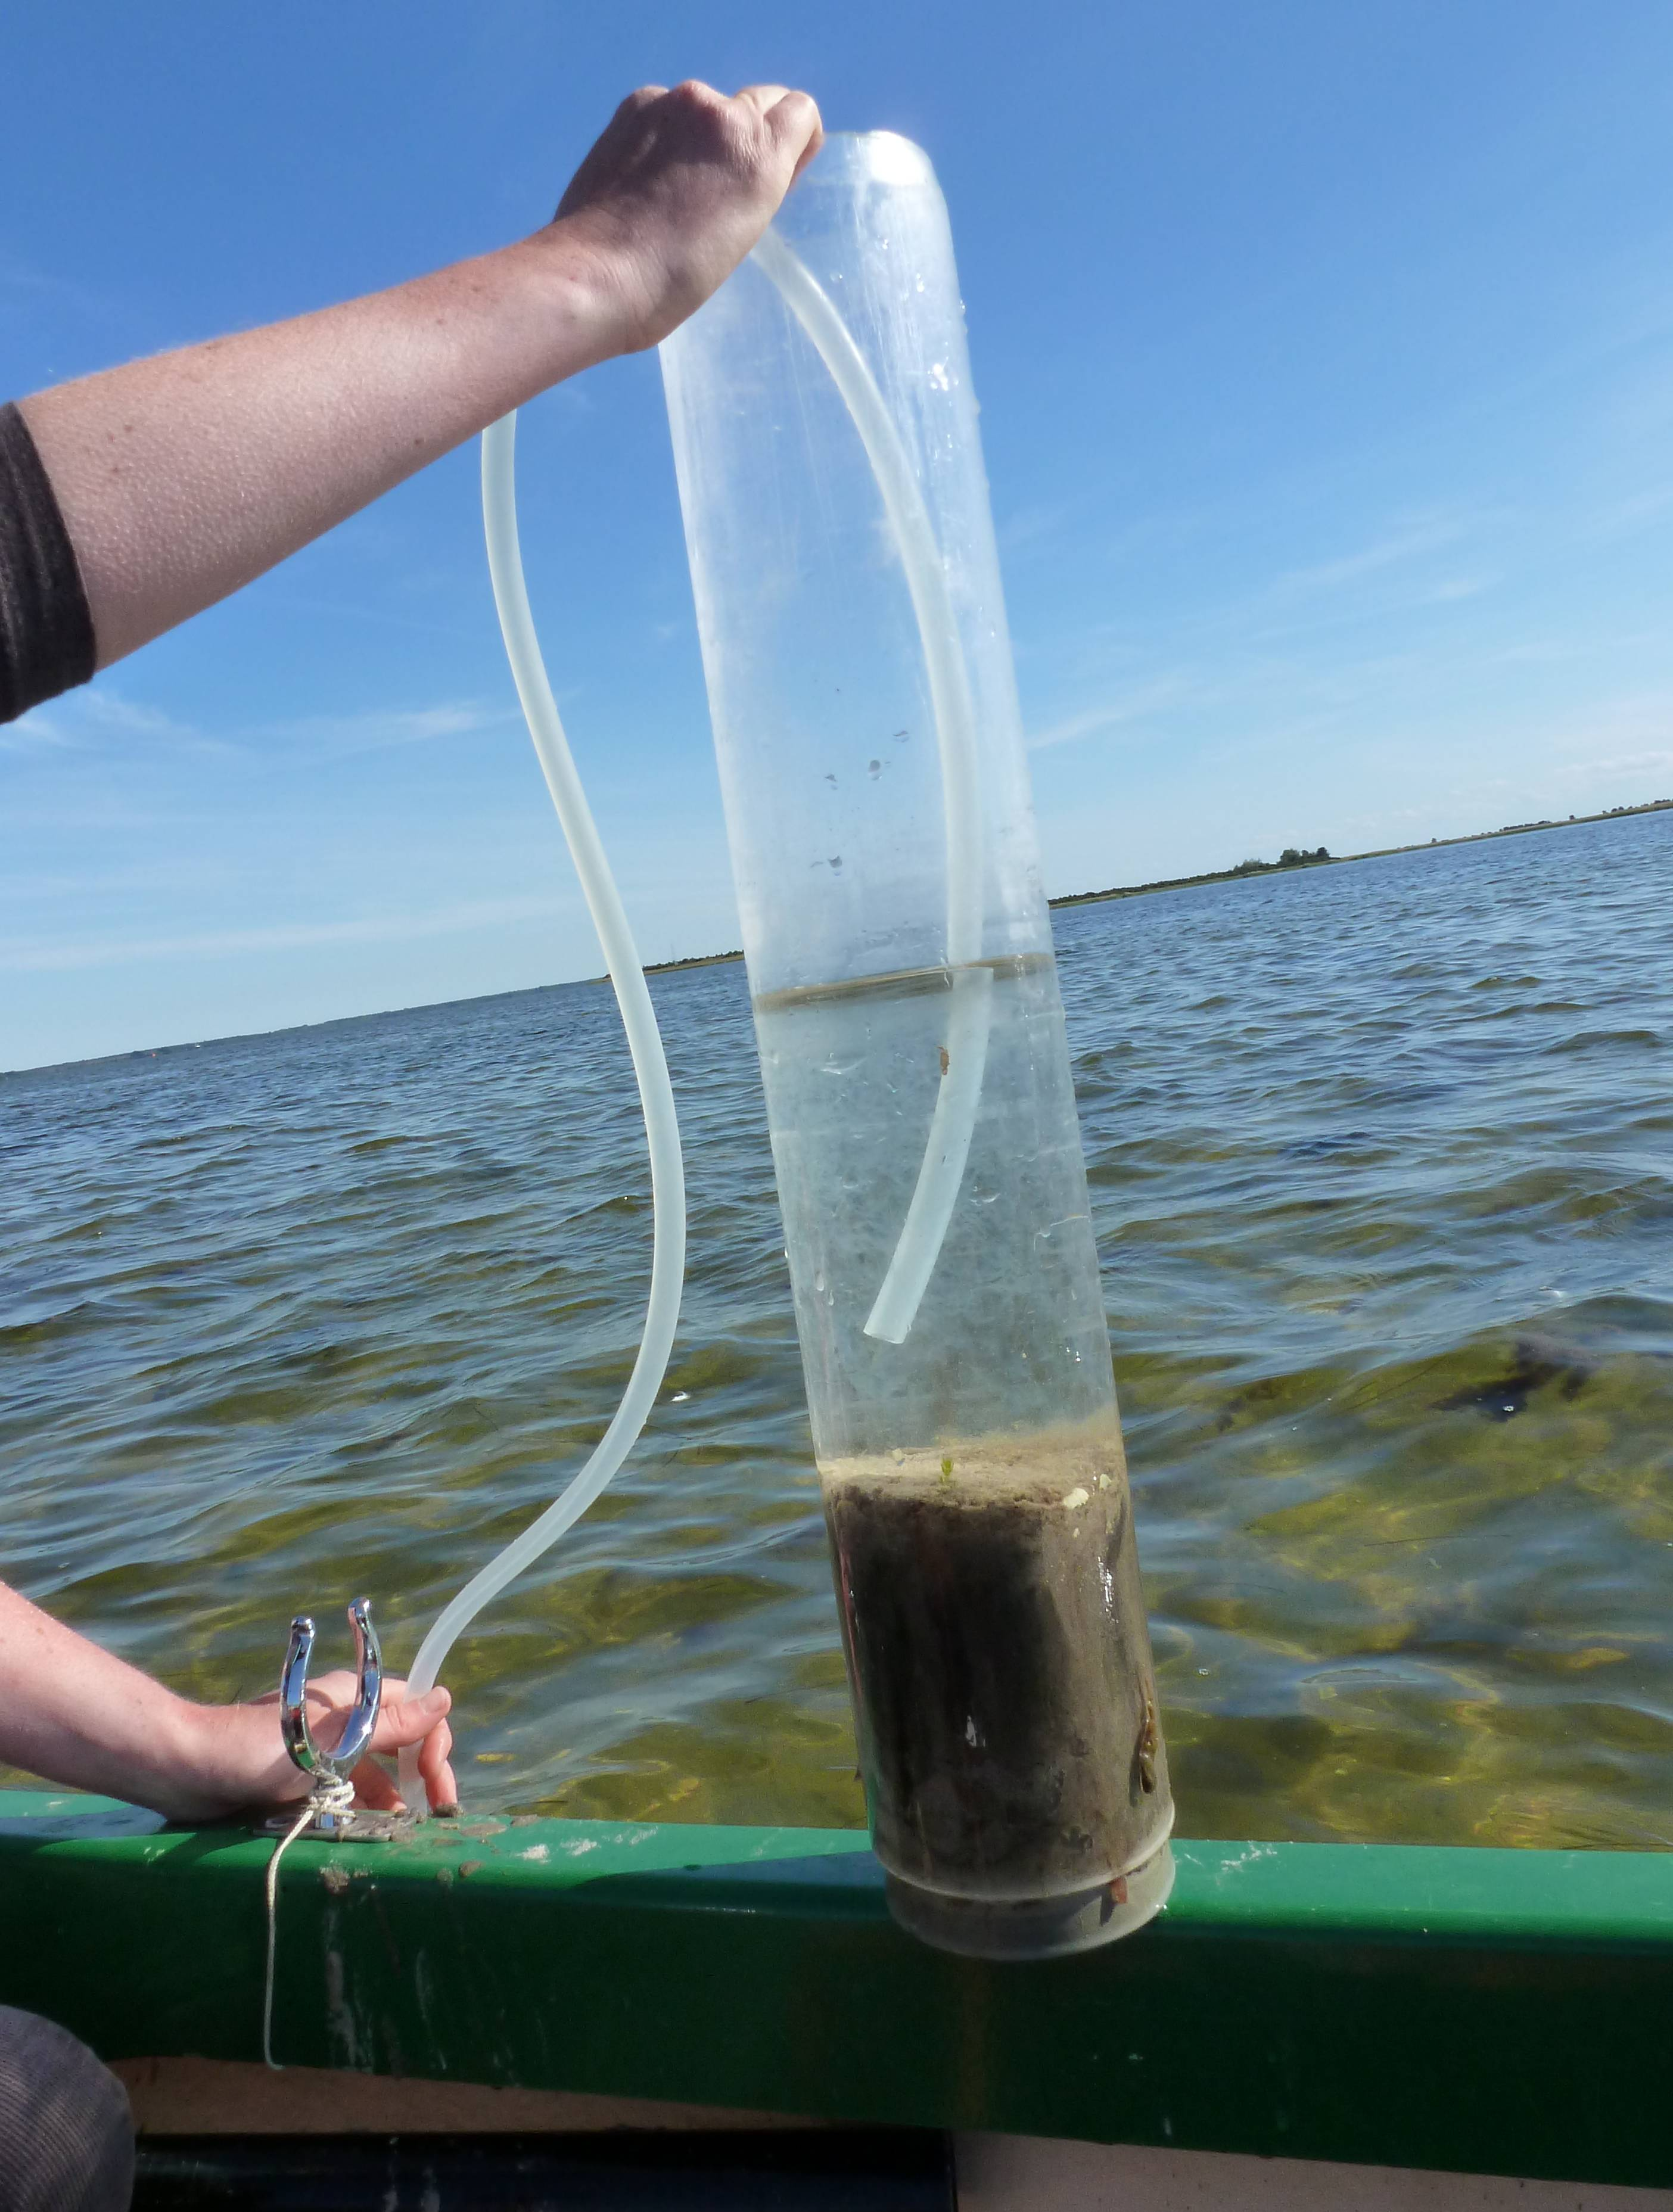
\includegraphics[height=55mm]{images/Fotos/Sedimentstechen.jpg}
\hspace*{-8mm}
\end{figure}
\end{column}
\begin{column}{6.4cm}
\begin{figure}
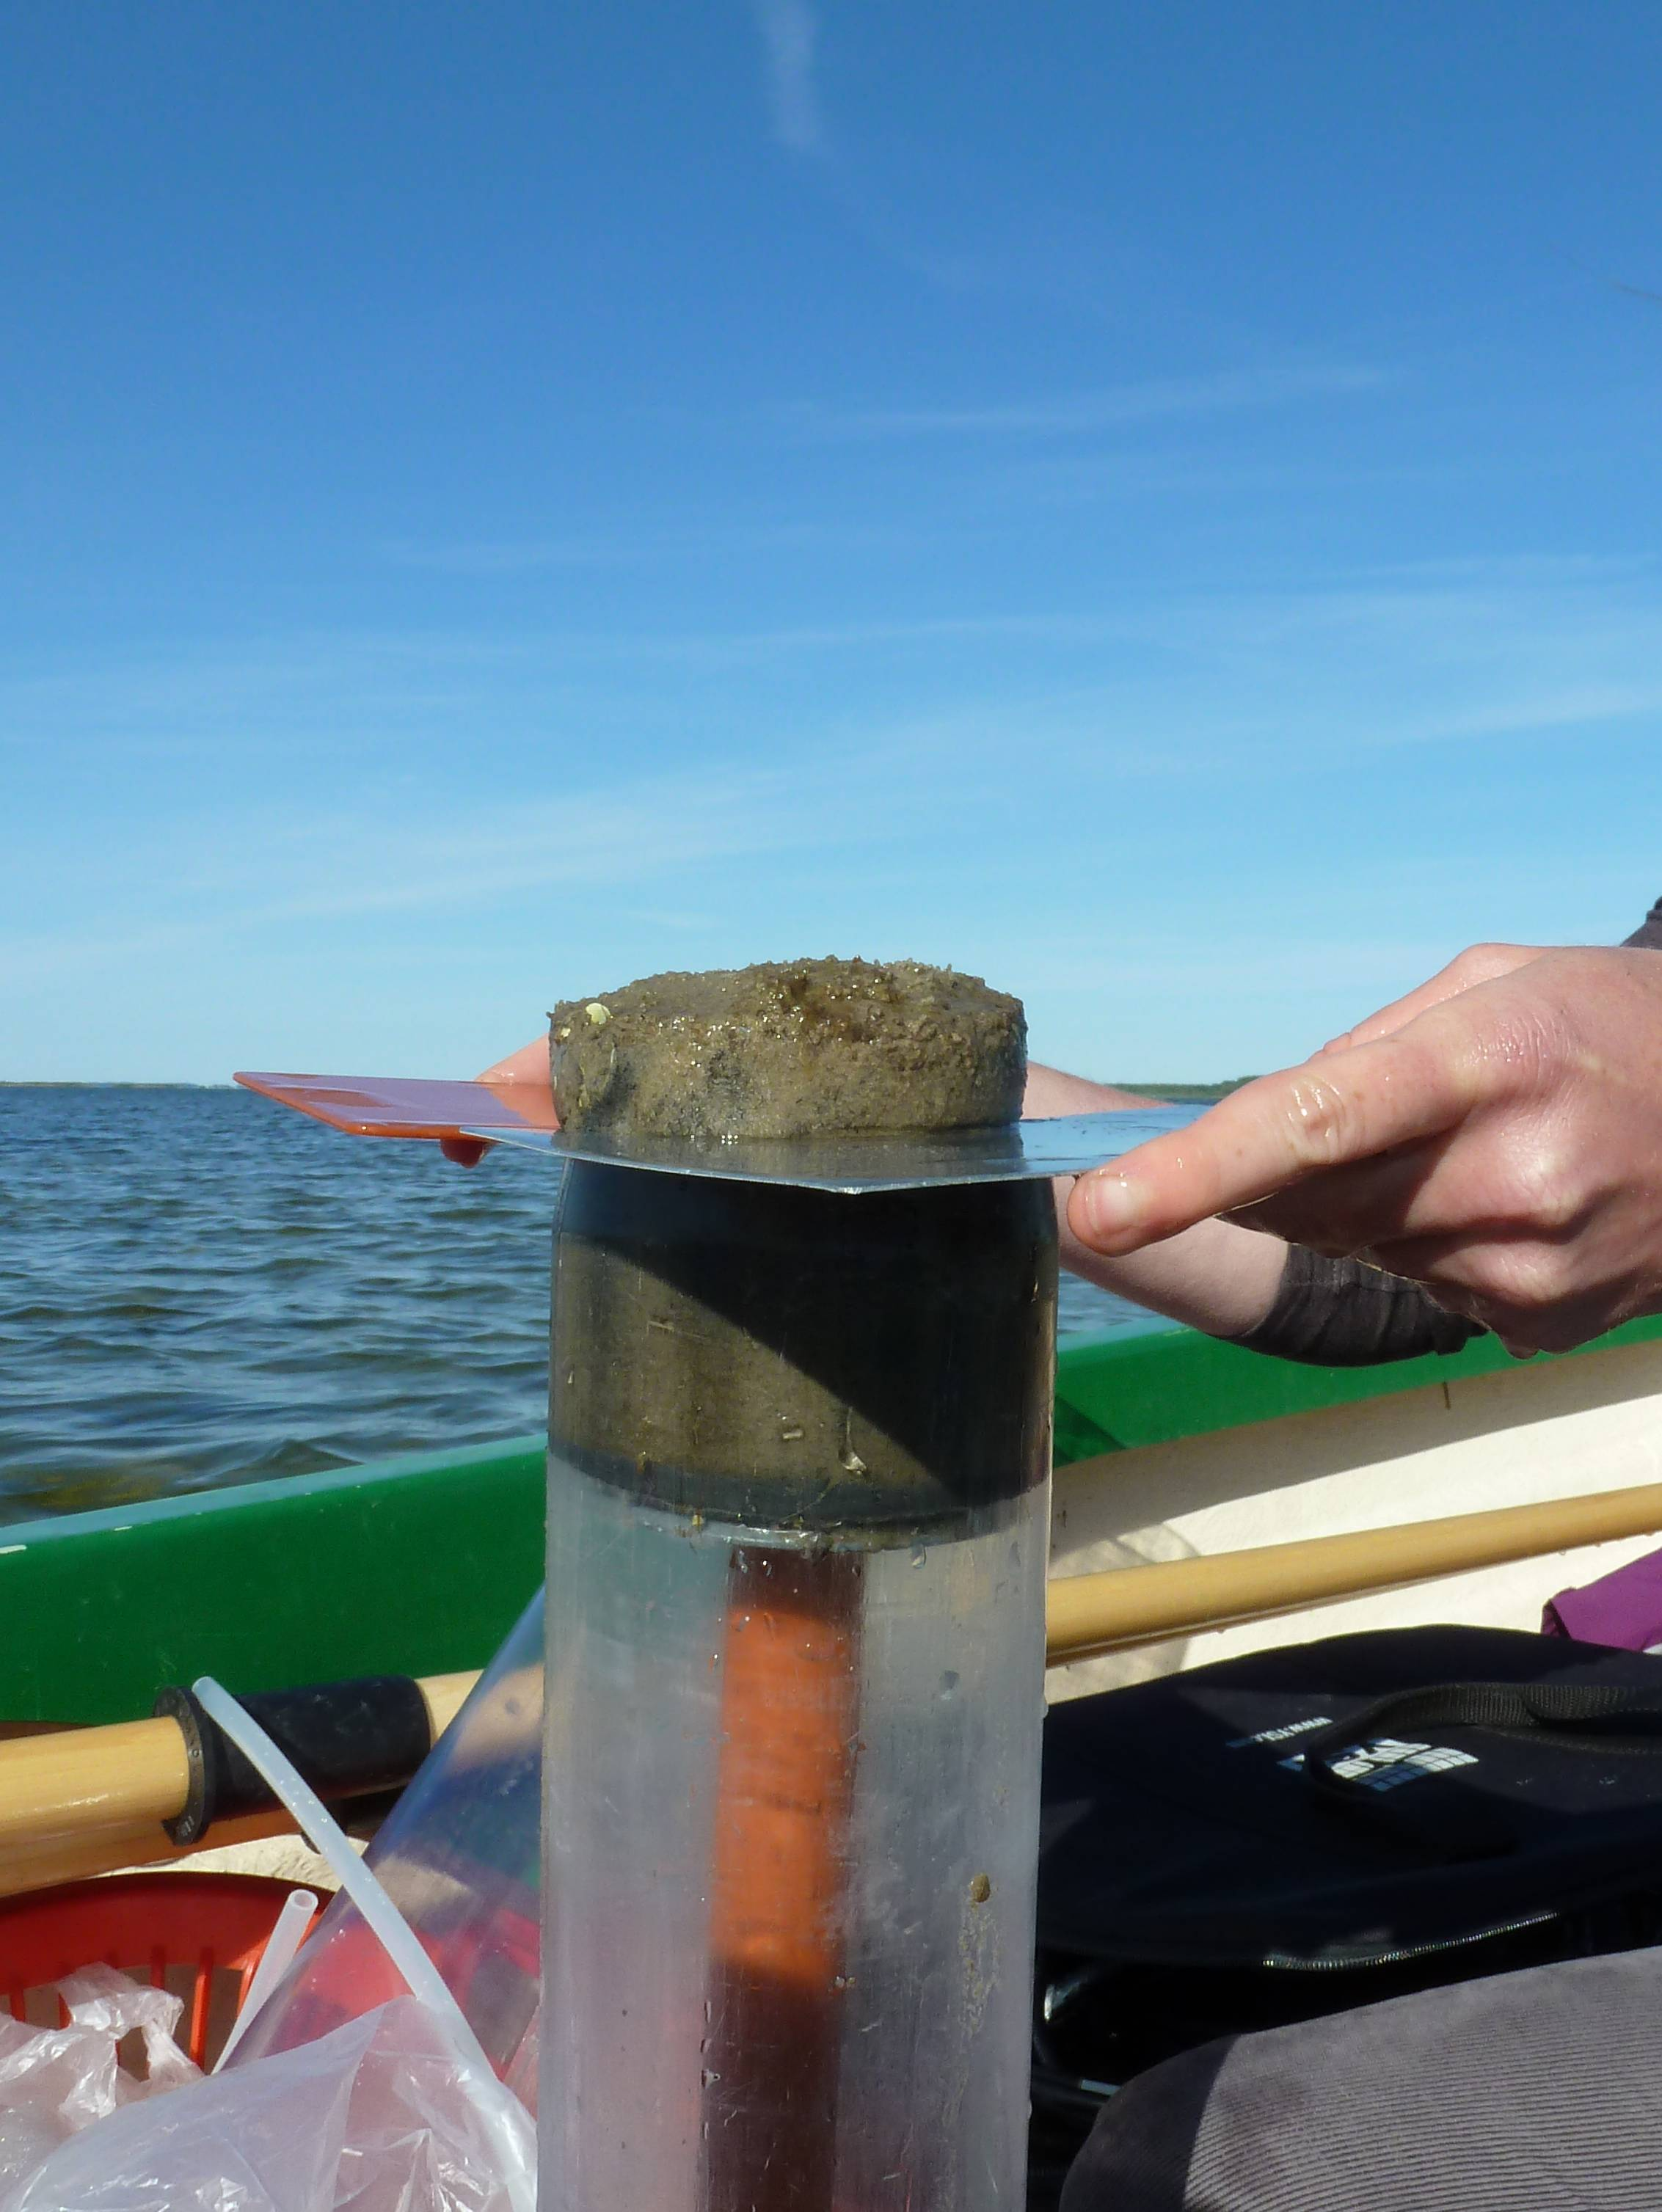
\includegraphics[height=55mm]{images/Fotos/Stempeln.jpg}
\hspace*{+8mm}
\end{figure}
\end{column}
\end{columns}
\end{frame}
\begin{frame}[t]
\begin{columns}[t]
\begin{column}{6.4cm}
\begin{figure}
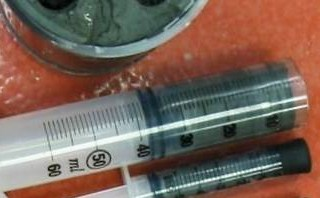
\includegraphics[height=25mm]{images/Fotos/spritze.jpg} {\small [1]}
\hspace*{-8mm}
\end{figure}
\begin{enumerate}
\item[1] Prozentualer Wassergehalt und organischer Gehalt
\end{enumerate}
\end{column}
\begin{column}{6.4cm}
\begin{figure}
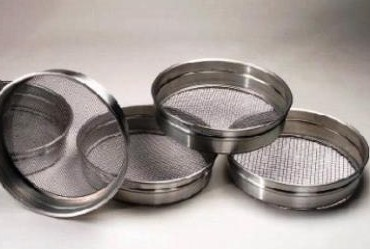
\includegraphics[height=25mm]{images/Fotos/Siebe2.jpeg} {\small [2]}
\hspace*{+8mm}
\end{figure}
\begin{enumerate}
\item[2] Korngrößenfraktionen
\begin{itemize}
\item 1000$ \mu$m 
\item 500$ \mu$m 
\item 250$ \mu$m 
\item 125$\mu$m 
\item 63$ \mu$m 
\end{itemize}
\item[3] Berechnung der $<63 \mu$m 
-Fraktion
\end{enumerate}
\end{column}
\end{columns}
\end{frame}

\subsection{Statistik}

\begin{frame}[t]
\frametitle{Statistische Auswertung}
\begin{figure}
\begin{flushleft}
Häufigkeit (\%)
\end{flushleft}
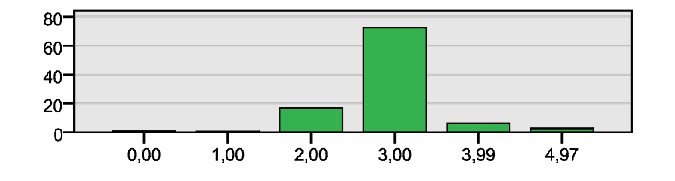
\includegraphics[height=30mm]{images/Fotos/bsp_kornverteilung.png}
\vspace*{-0.76cm}
\end{figure}
\begin{flushright}
Korngrößenklasse ($ \Phi $)
\end{flushright}
\begin{itemize}
\setlength{\itemindent}{+5.5cm} 
\item[Unterschiede zwischen $ +M $ und $ -M $:] Mann-Whithney-Test
\item[Unterschiede im Jahresverlauf:] Kruskal-Wallis-Test, 
\item[] Dunn's-Test 
\end{itemize}
\end{frame}


\section{Ergebnisse und Diskussion}
\subsection{Vegetation}

\begin{frame}
\frametitle{Grieben (+M)}
\begin{columns}
\begin{column}{7.0cm}
\begin{figure}
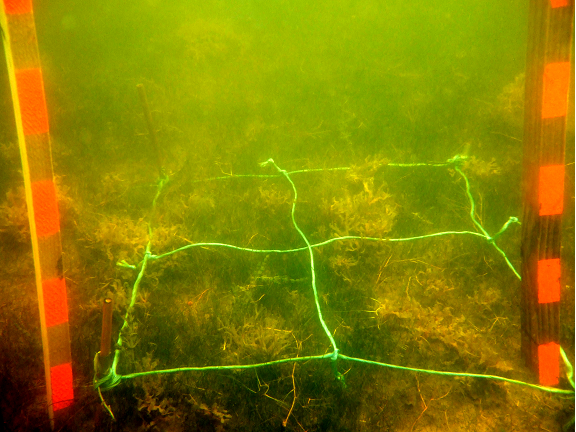
\includegraphics[height=0.5\textheight]{images/plotpictures/Bsp_G+M}
\hspace*{-9mm}
\end{figure}
\end{column}
\begin{column}{5.8cm}
\begin{figure}
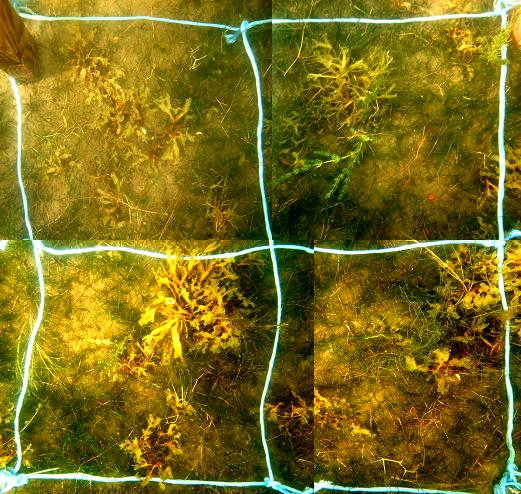
\includegraphics[height=0.5\textheight]{images/Fotos/griebenvonoben.jpg}
\hspace*{+9mm}
\end{figure}
\end{column}
\end{columns}
\end{frame}

\begin{frame}
\frametitle{Grieben (+M)}
\begin{columns}
\begin{column}{4.8cm}
\begin{figure}
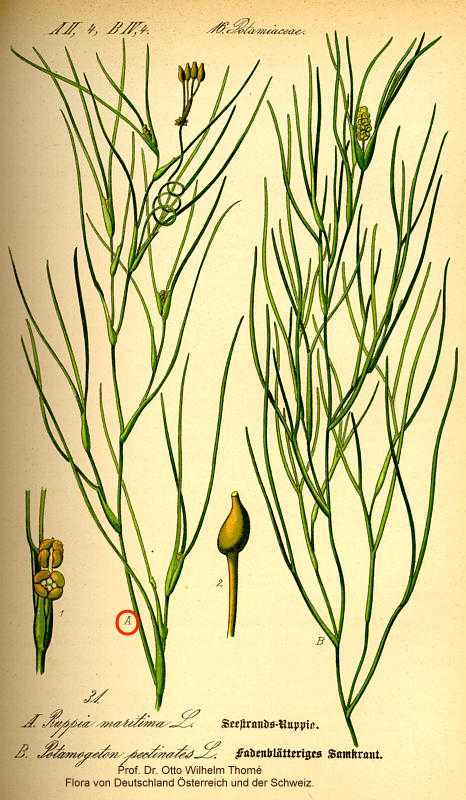
\includegraphics[width=0.75\textwidth]{images/Fotos/ruppia.jpg} {\small [3]}
\end{figure}
\end{column}
\begin{column}{8.0cm}
\begin{figure}
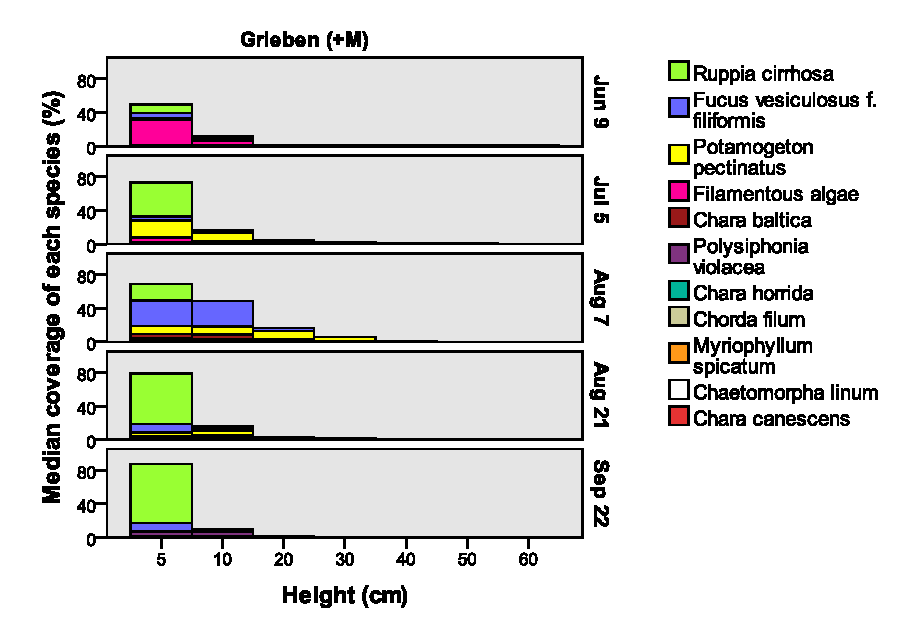
\includegraphics[width=\textwidth]{images/Wuchshoehenkartierung/Grieben+M1.eps}
\end{figure}
\end{column}
\end{columns}
\end{frame}

\begin{frame}
\frametitle{Vitte (+M)}
\begin{columns}
\begin{column}{7.0cm}
\begin{figure}
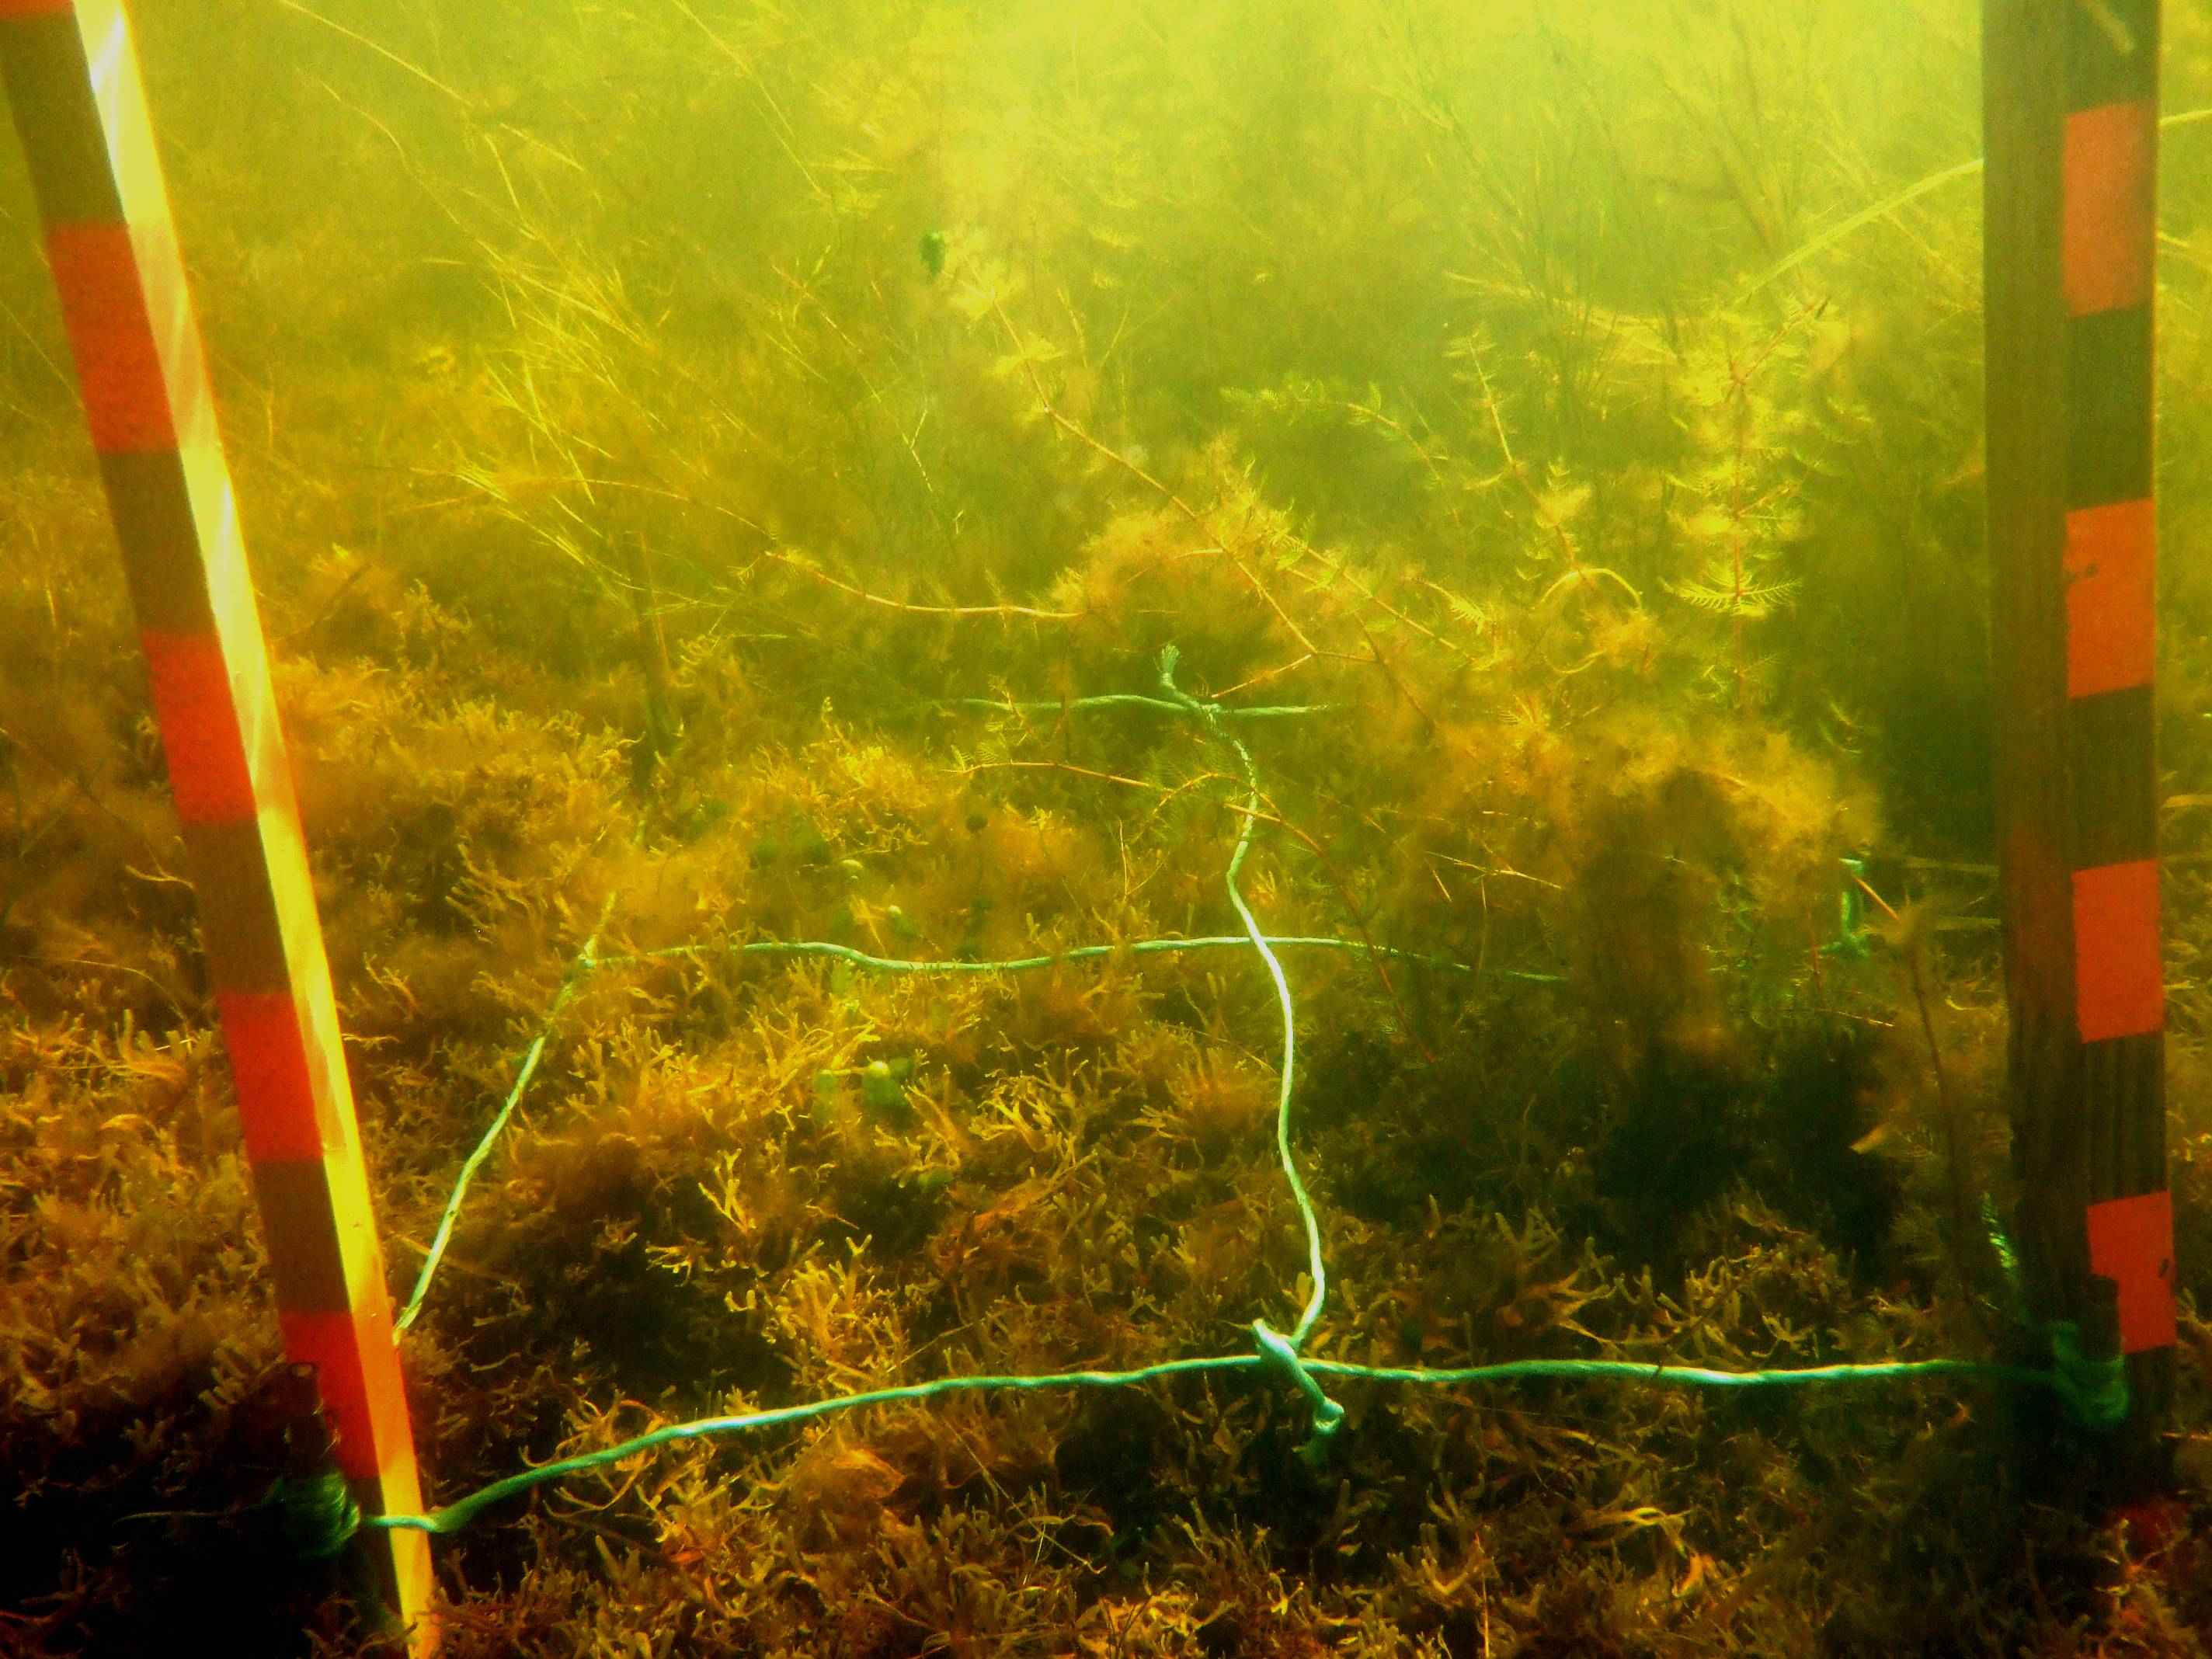
\includegraphics[height=0.5\textheight]{images/plotpictures/BSP_V+M}
\hspace*{-9mm}
\end{figure}
\end{column}
\begin{column}{5.8cm}
\begin{figure}
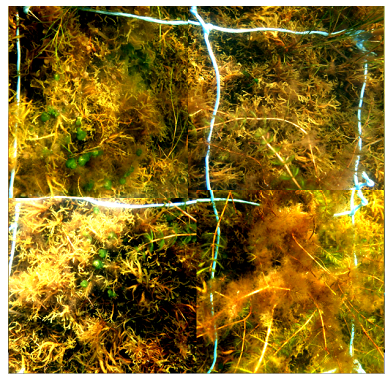
\includegraphics[height=0.5\textheight]{images/plotpictures/V+M.png}
\hspace*{+9mm}
\end{figure}
\end{column}
\end{columns}
\end{frame}

\begin{frame}
\frametitle{Vitte (+M)}
\begin{columns}
\begin{column}{4.8cm}
\begin{figure}
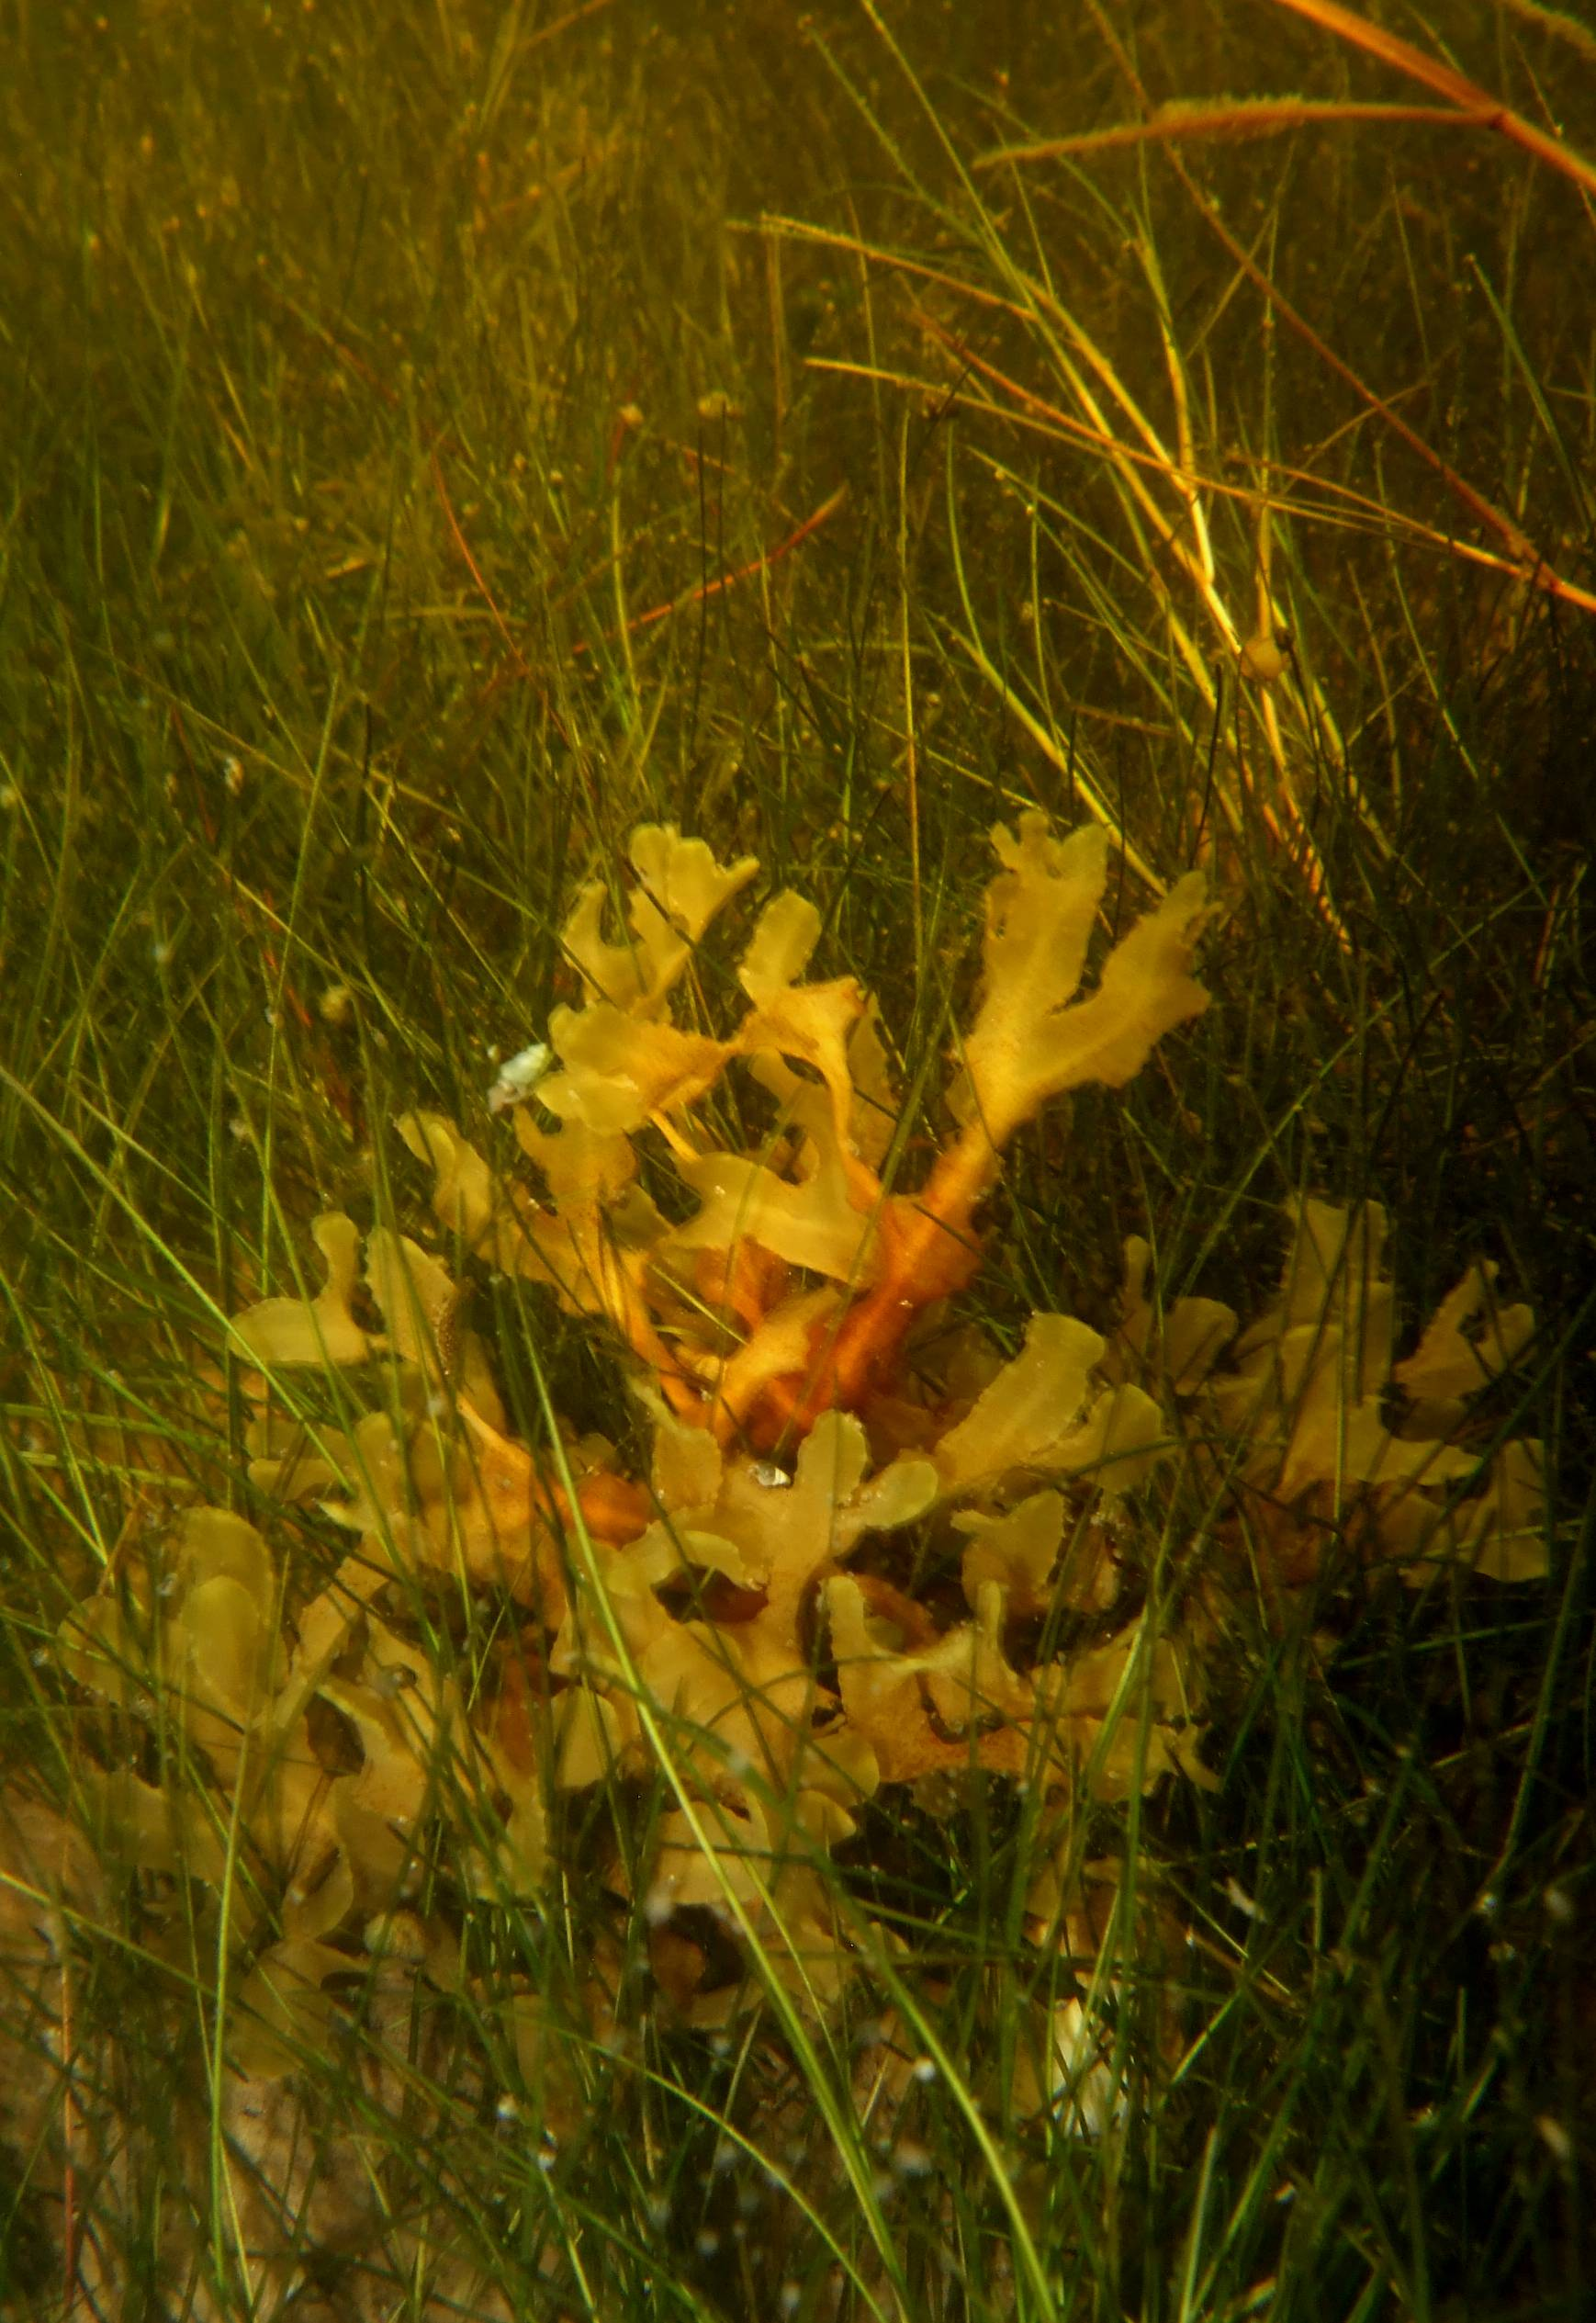
\includegraphics[width=0.7\textwidth]{images/Fotos/DSCF0799.JPG} 
\end{figure}
\end{column}
\begin{column}{8.0cm}
\begin{figure}
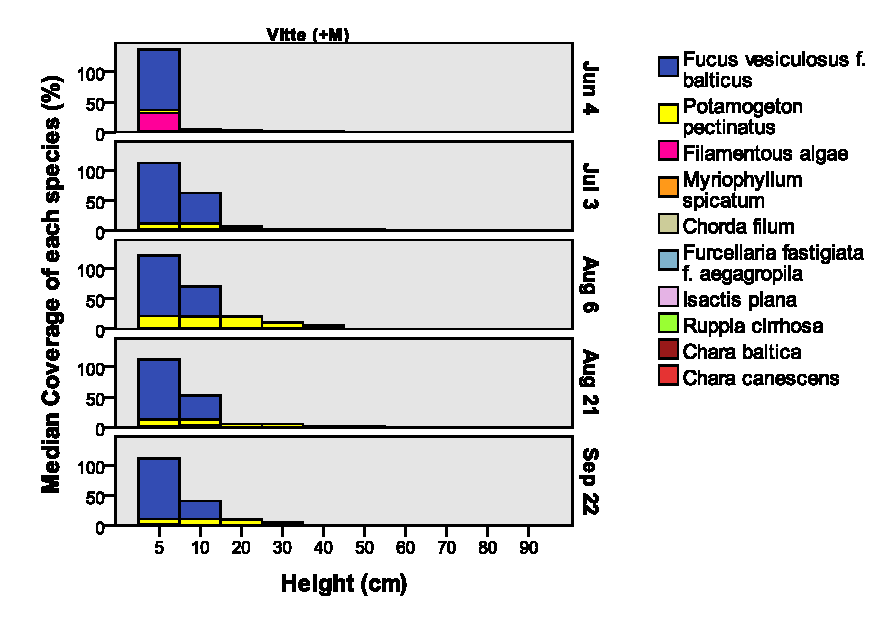
\includegraphics[width=\textwidth]{images/Wuchshoehenkartierung/Vitte+Mb1.eps}
\end{figure}
\end{column}
\end{columns}
\end{frame}

\begin{frame}
\frametitle{Spärlich bewachsene Standorte}
\begin{columns}
\begin{column}{5.5cm}
\begin{figure}
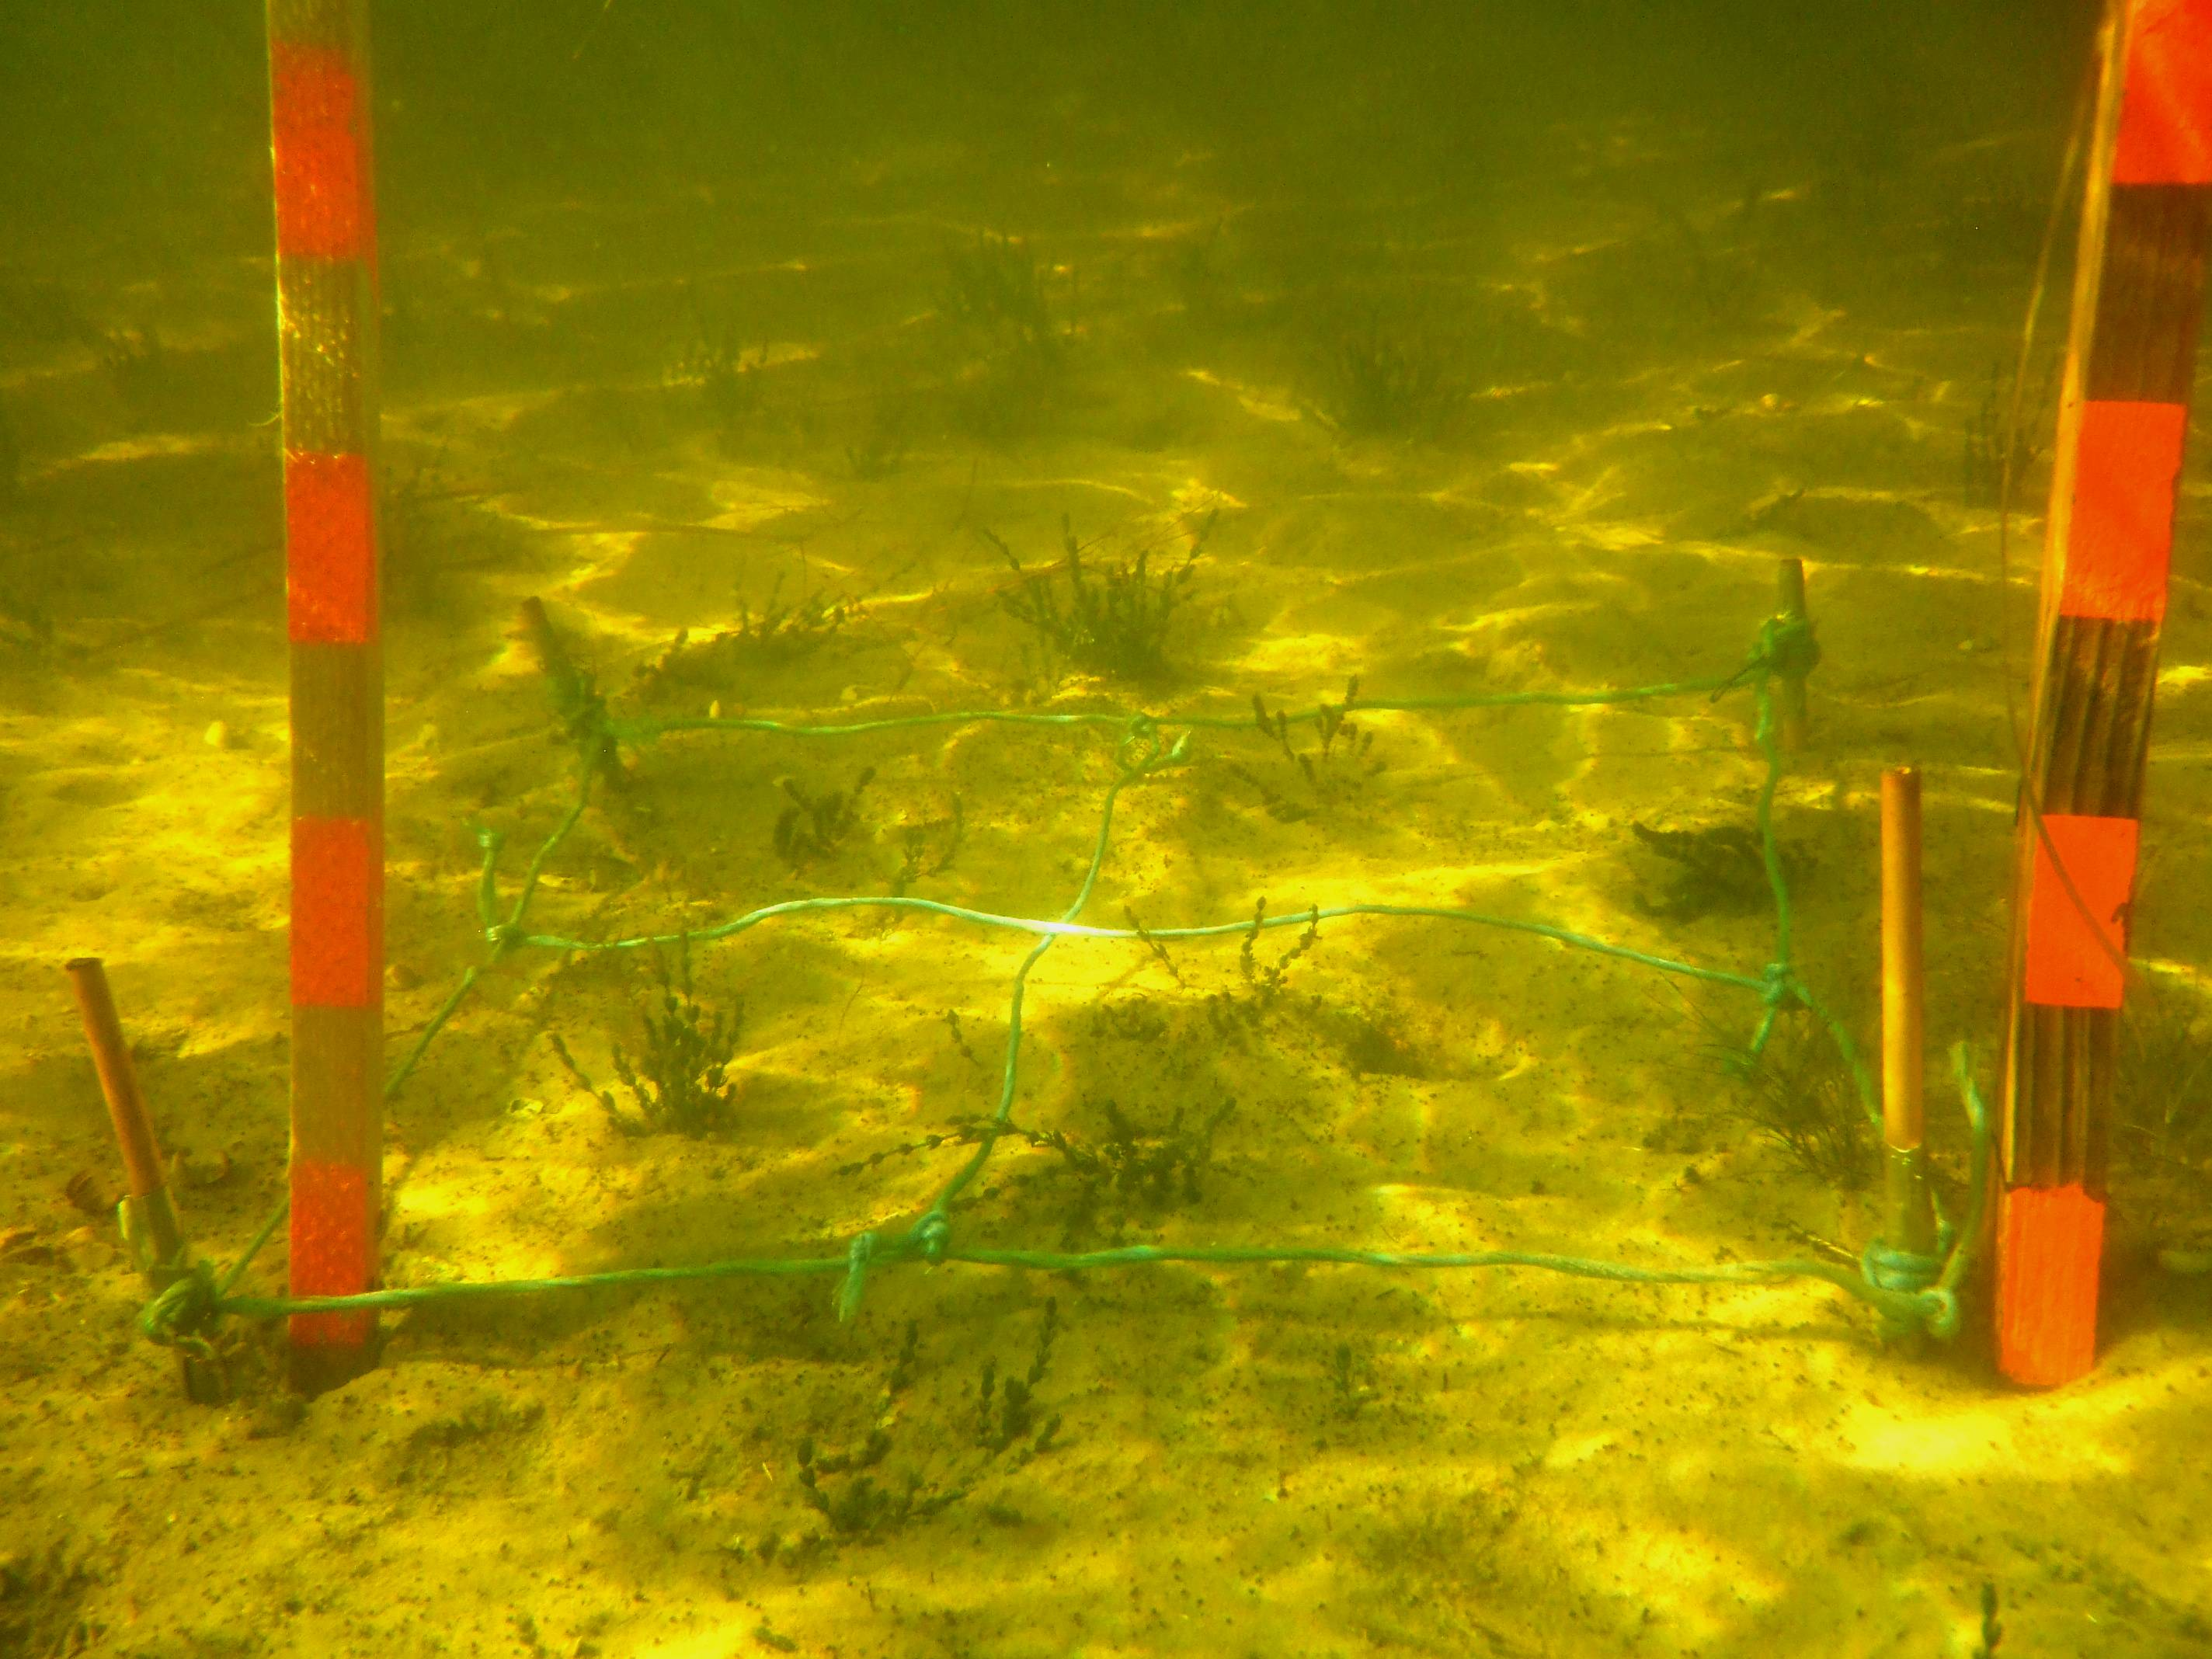
\includegraphics[width=\textwidth]{images/plotpictures/Bsp_V-M}
\end{figure}
\end{column}
\begin{column}{5.5cm}
\begin{figure}
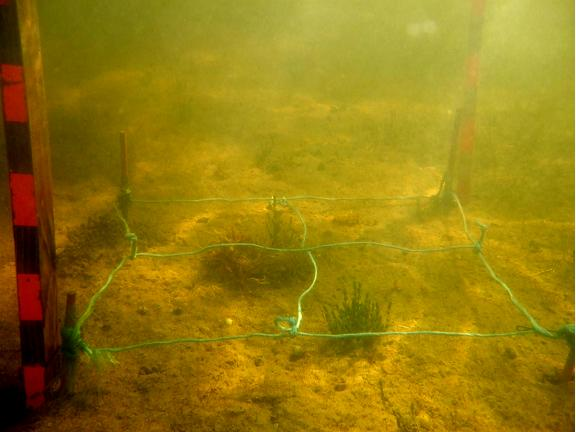
\includegraphics[width=\textwidth]{images/plotpictures/Bsp_G-M}
\end{figure}
\end{column}
\end{columns}
\end{frame}

\begin{frame}
\frametitle{Grieben (-M)}
\begin{columns}
\begin{column}{4.8cm}
\begin{figure}
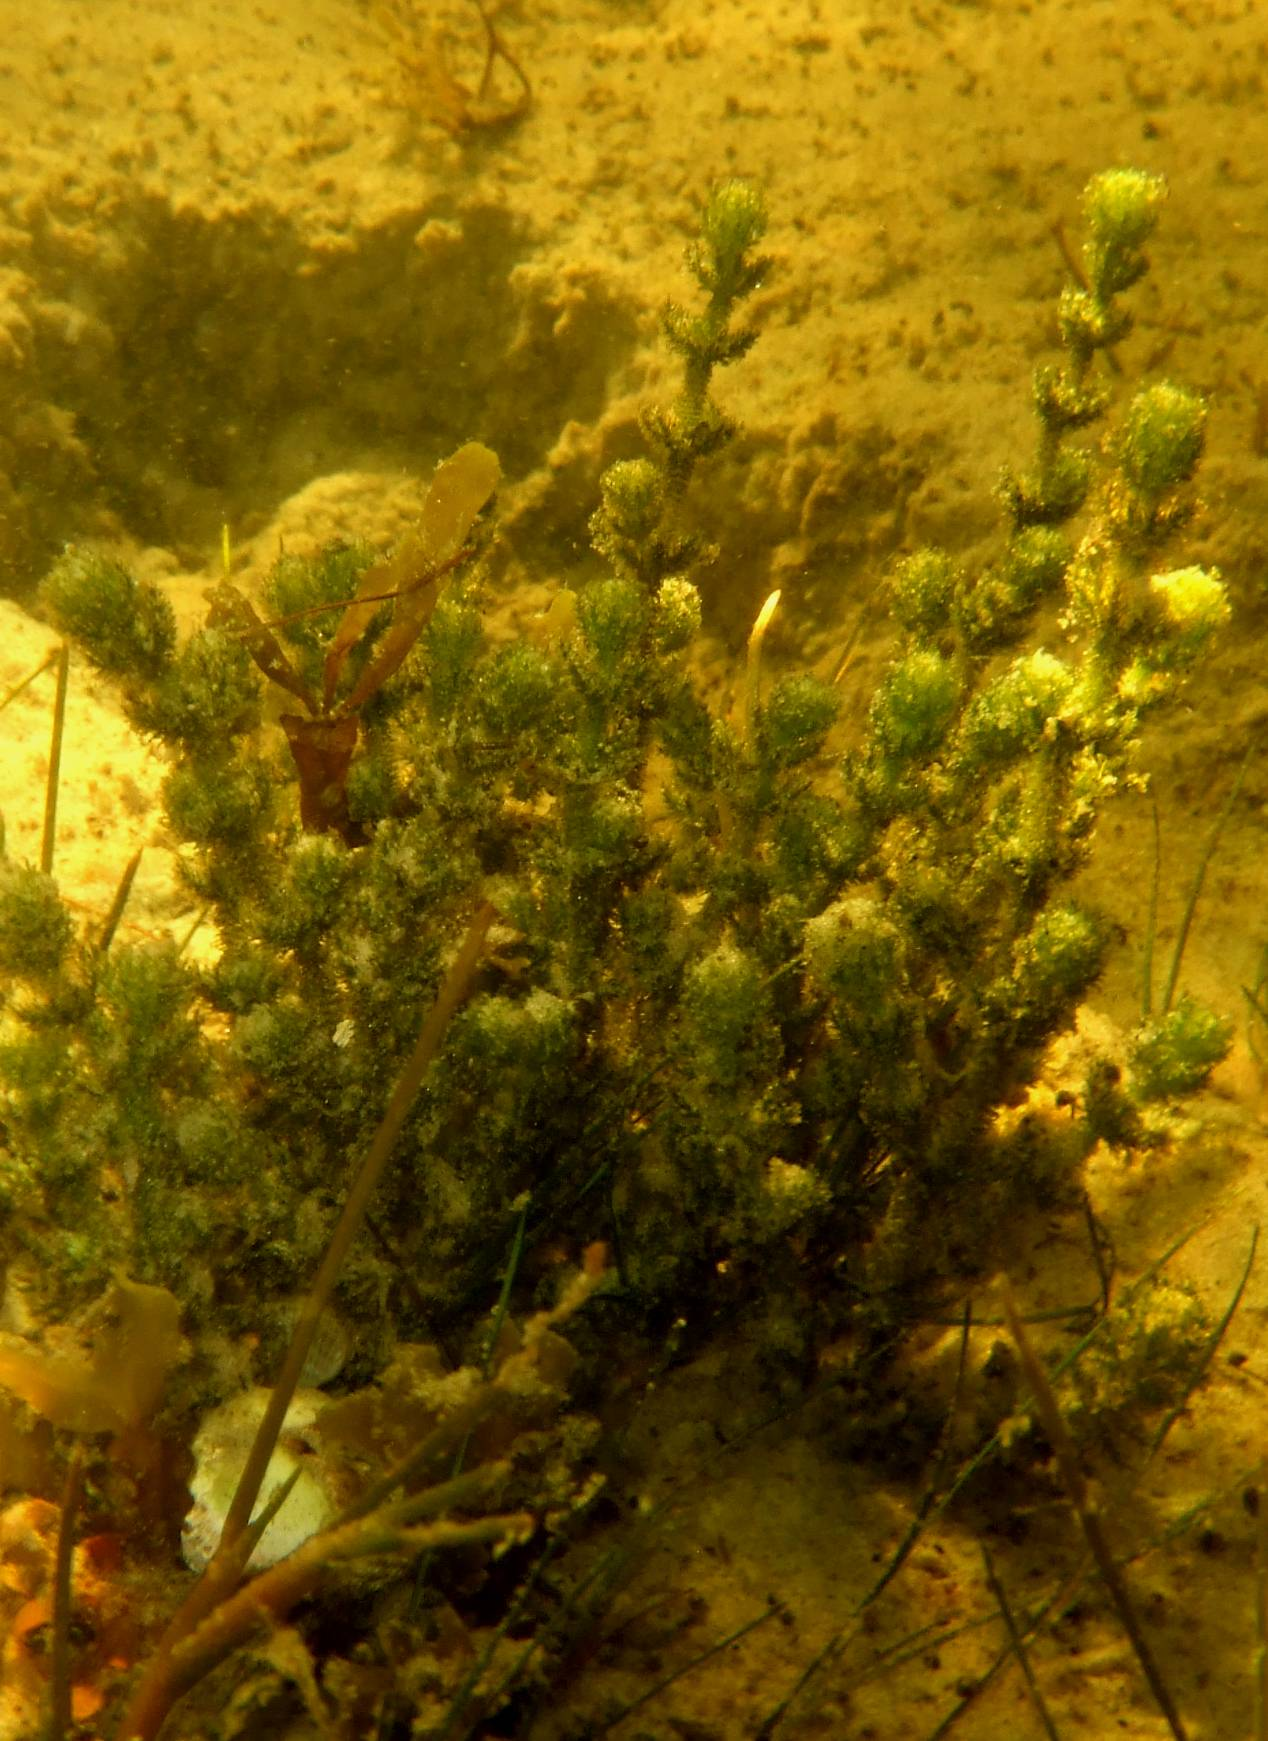
\includegraphics[width=0.7\textwidth]{images/Fotos/DSCF0876.JPG}
\end{figure}
\end{column}
\begin{column}{8.0cm}
\begin{figure}
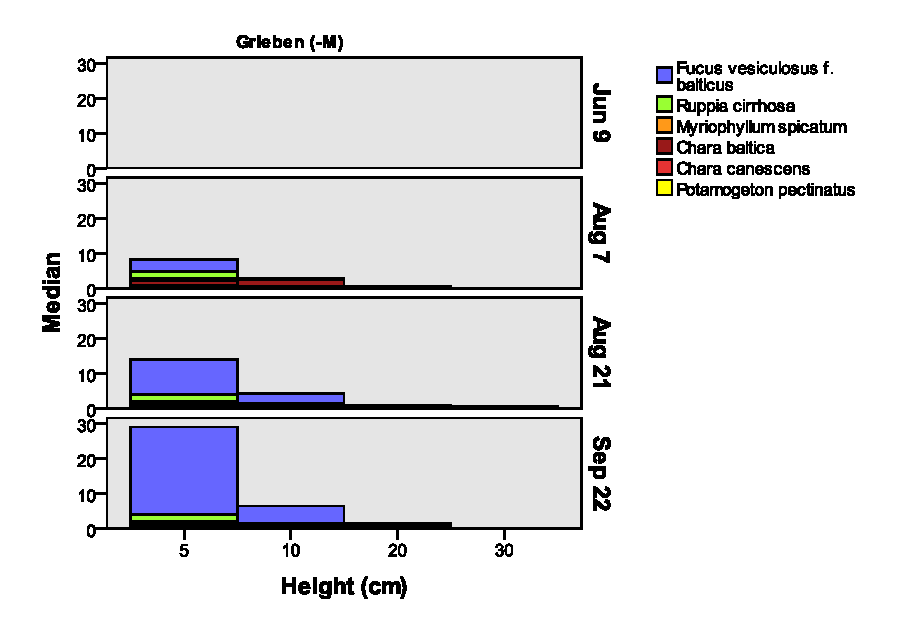
\includegraphics[width=\textwidth]{images/Wuchshoehenkartierung/Grieben-M1.eps}
\end{figure}
\end{column}
\end{columns}
\end{frame}

\begin{frame}
\frametitle{Vitte (-M)}
\begin{columns}
\begin{column}{4.8cm}

\end{column}
\begin{column}{8.0cm}
\begin{figure}
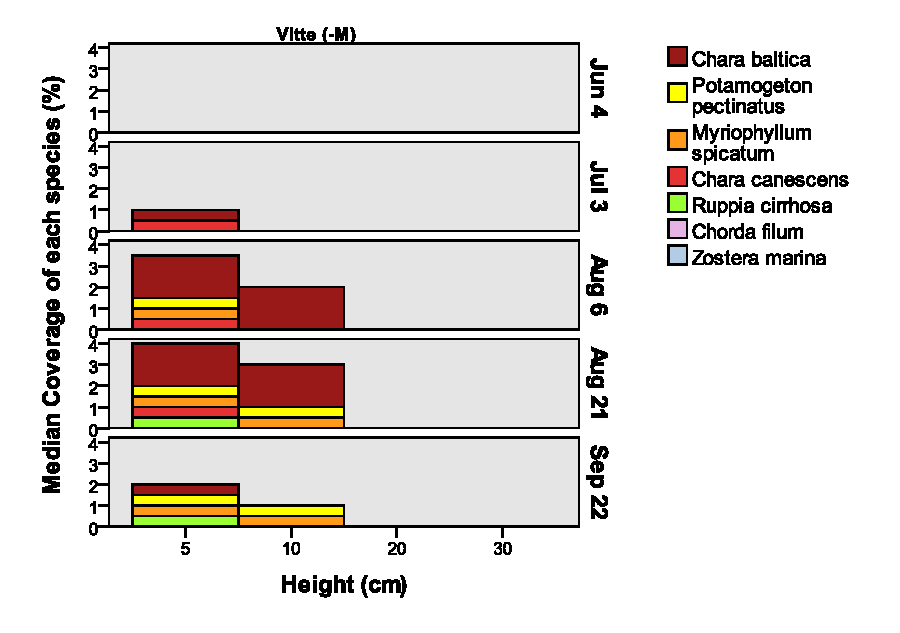
\includegraphics[width=\textwidth]{images/Wuchshoehenkartierung/Vitte-M1.eps}
\end{figure}
\end{column}
\end{columns}
\end{frame}

\begin{frame}
\frametitle{Bedeckung mit Makrophytobenthos und PVI in Grieben}
\begin{columns}
\begin{column}{5.5cm}
\begin{figure}
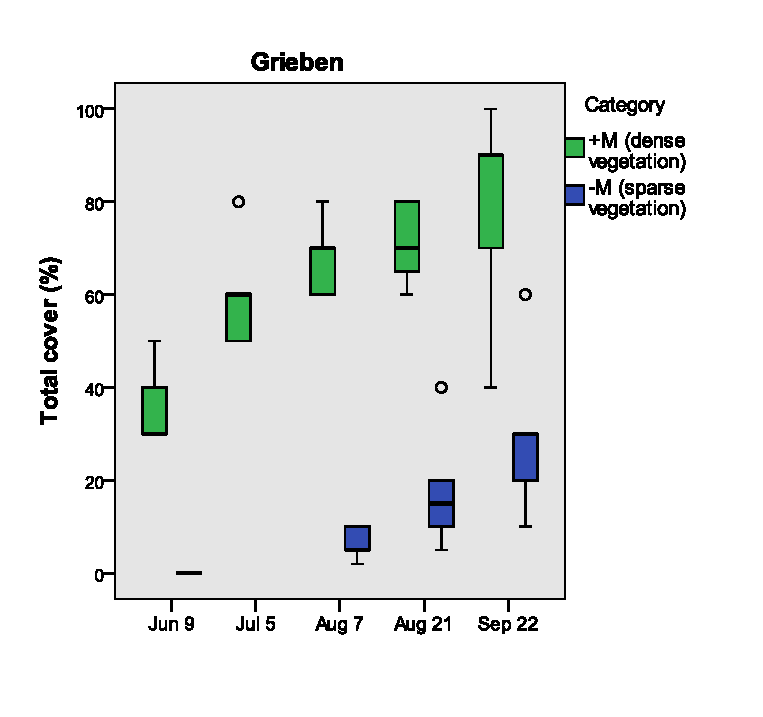
\includegraphics[width=\textwidth]{images/total_cover/total_cover2.eps}
\end{figure}
\end{column}
\begin{column}{5.5cm}
\begin{figure}
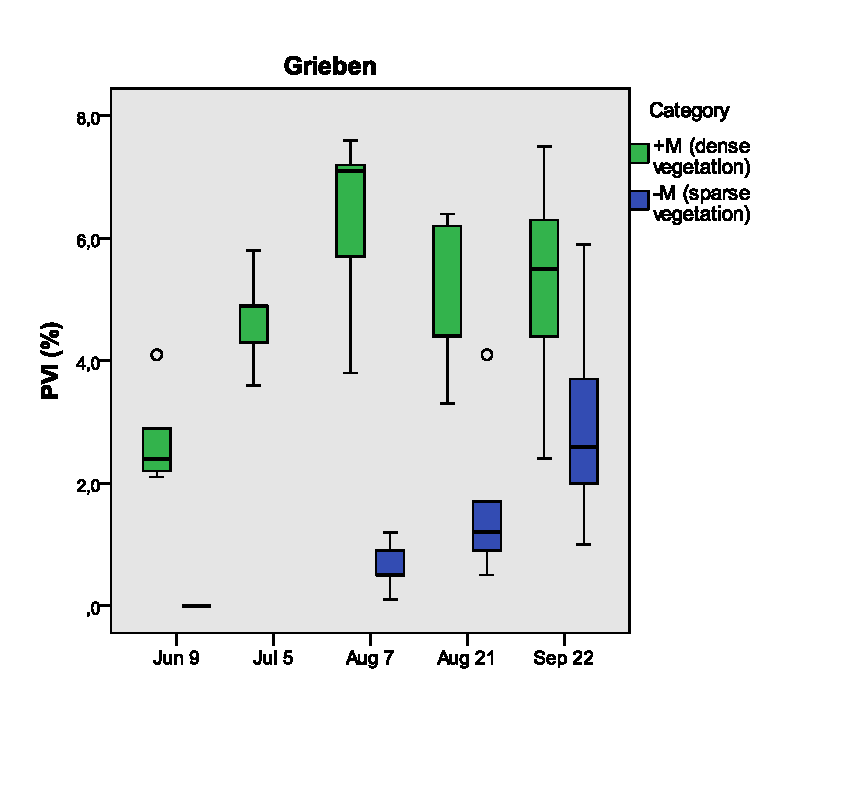
\includegraphics[width=\textwidth]{images/pvi/boxplot_pvi2.eps}
\end{figure}
\end{column}
\end{columns}
\end{frame}

\subsection{Deckung und PVI}
\begin{frame}
\frametitle{Bedeckung mit Makrophytobenthos und PVI in Vitte}
\begin{columns}
\begin{column}{5.5cm}
\begin{figure}
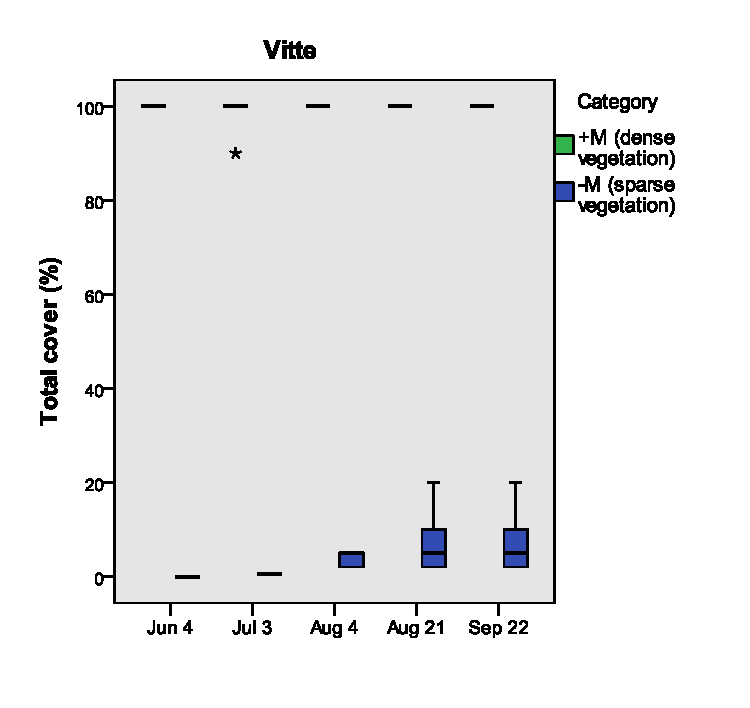
\includegraphics[width=\textwidth]{images/total_cover/total_cover1.eps}
\end{figure}
\end{column}
\begin{column}{5.5cm}
\begin{figure}
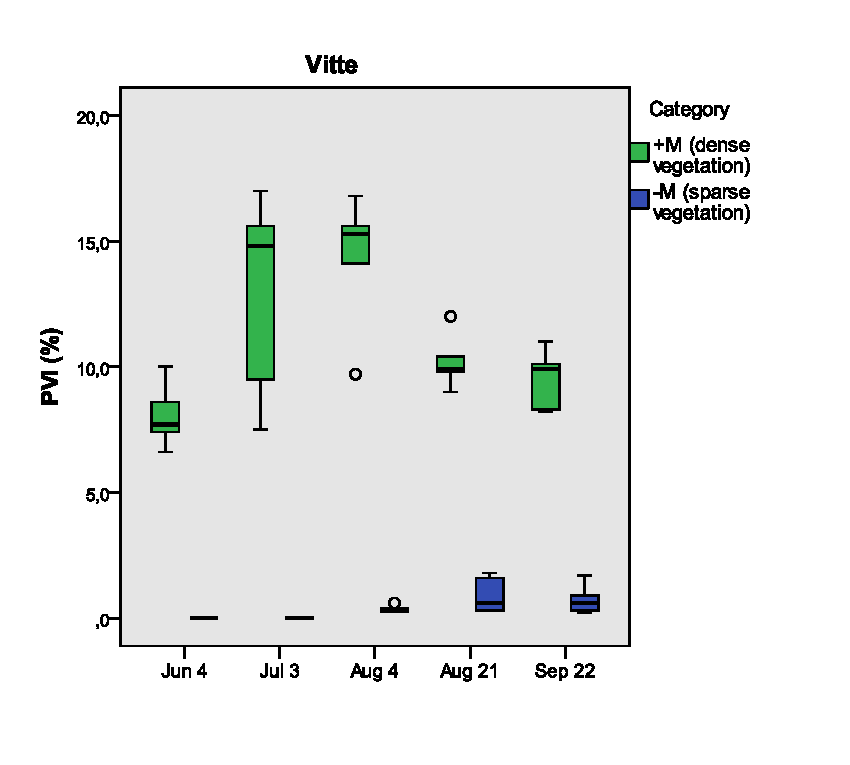
\includegraphics[width=\textwidth]{images/pvi/boxplot_pvi1.eps}
\end{figure}
\end{column}
\end{columns}
\end{frame}

\subsection{Sediment}

\begin{frame}
\frametitle{Korngrößenverteilungen in Grieben}
\begin{columns}
\begin{column}{5.5cm}
+M
\begin{figure}
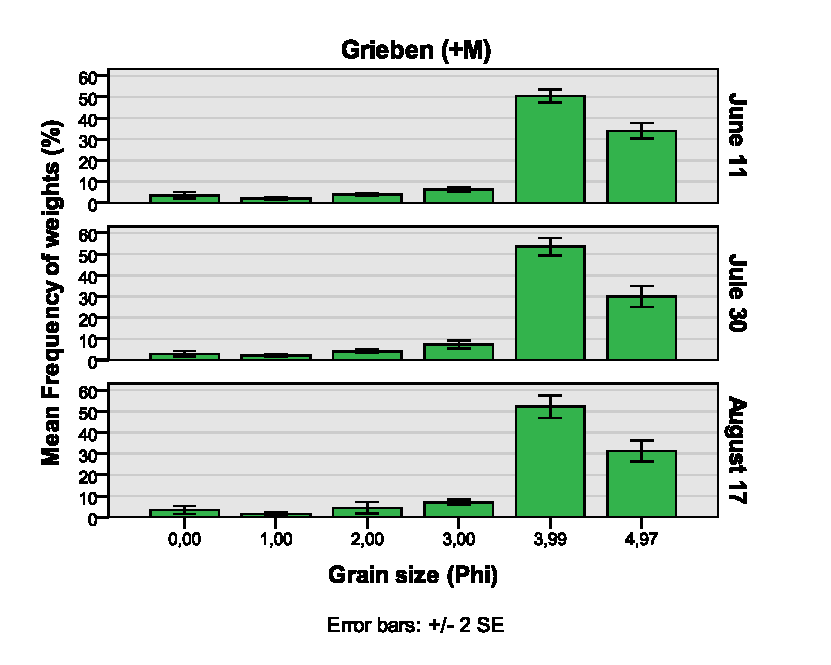
\includegraphics[width=\textwidth]{images/grainsize/sediment_im_jahr3.eps}
\end{figure}
\end{column}
\begin{column}{5.5cm}
-M
\begin{figure}
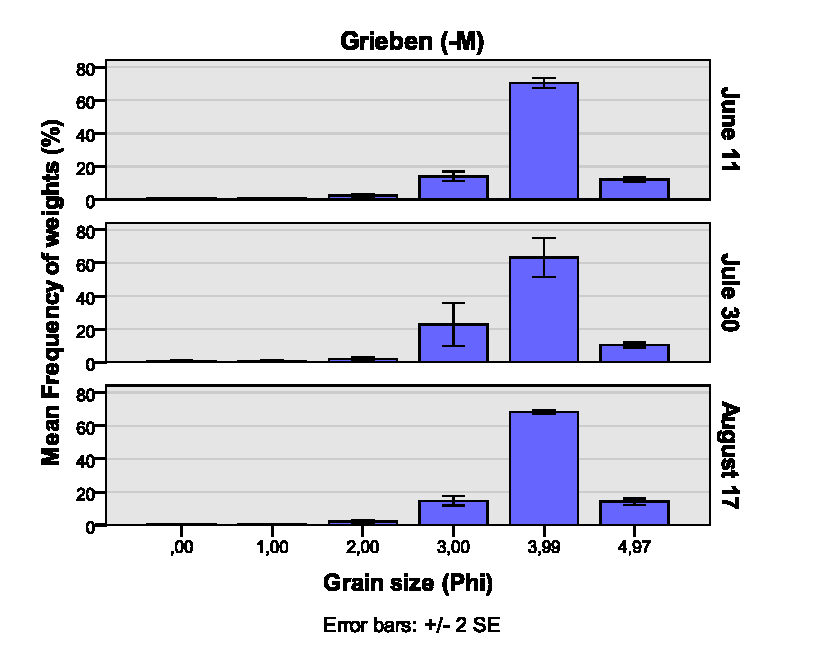
\includegraphics[width=\textwidth]{images/grainsize/sediment_im_jahr4.eps}
\end{figure}
\end{column}
\end{columns}
\end{frame}

\begin{frame}
\frametitle{Korngrößenverteilungen in Vitte}
\begin{columns}
\begin{column}{5.5cm}
+M
\begin{figure}
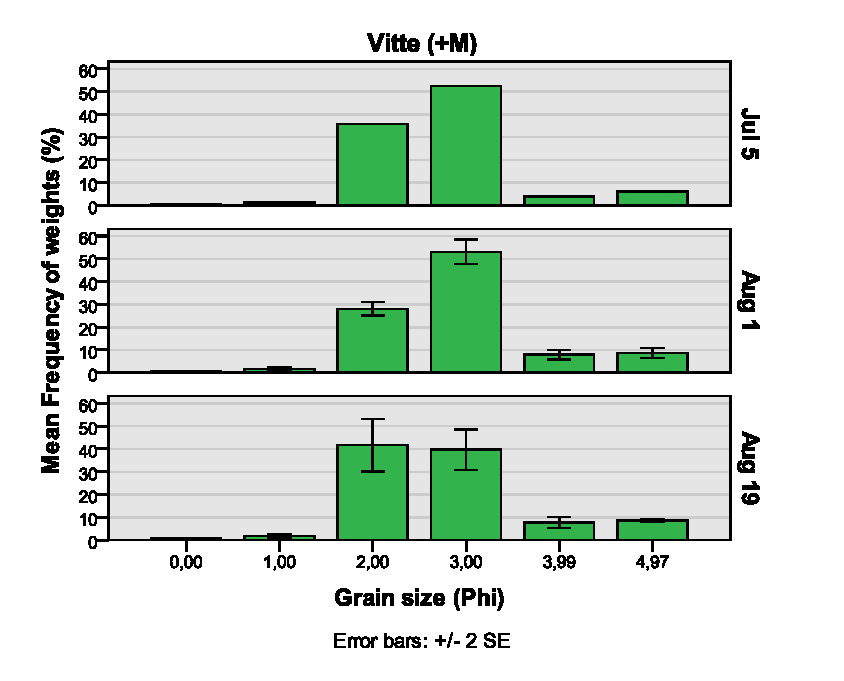
\includegraphics[width=\textwidth]{images/grainsize/sediment_im_jahr1.eps}
\end{figure}
\end{column}
\begin{column}{5.5cm}
-M
\begin{figure}
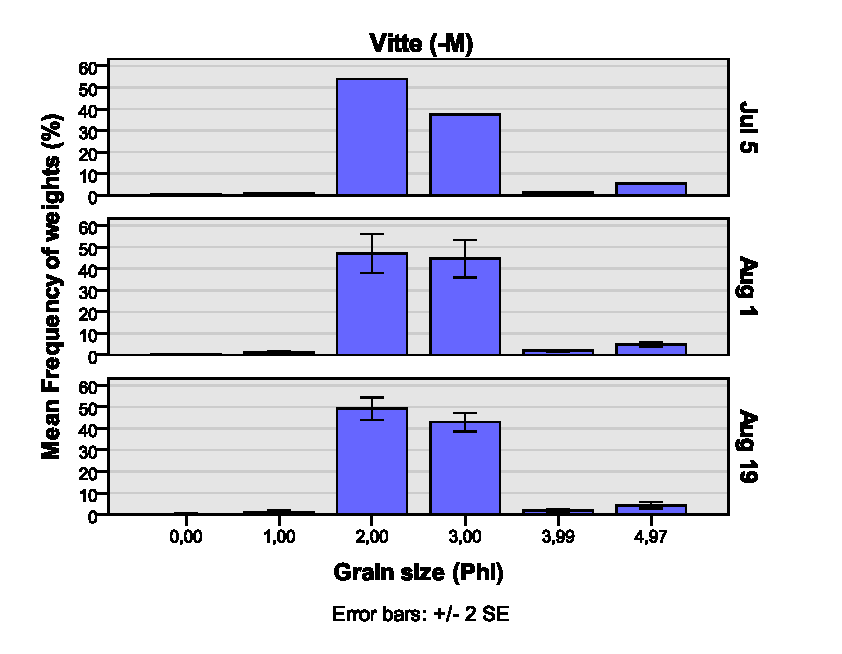
\includegraphics[width=\textwidth]{images/grainsize/sediment_im_jahr2.eps}
\end{figure}
\end{column}
\end{columns}
\end{frame}

\begin{frame}
\begin{columns}
\begin{column}{5.5cm}
Feinpartikulärer Anteil
\begin{figure}
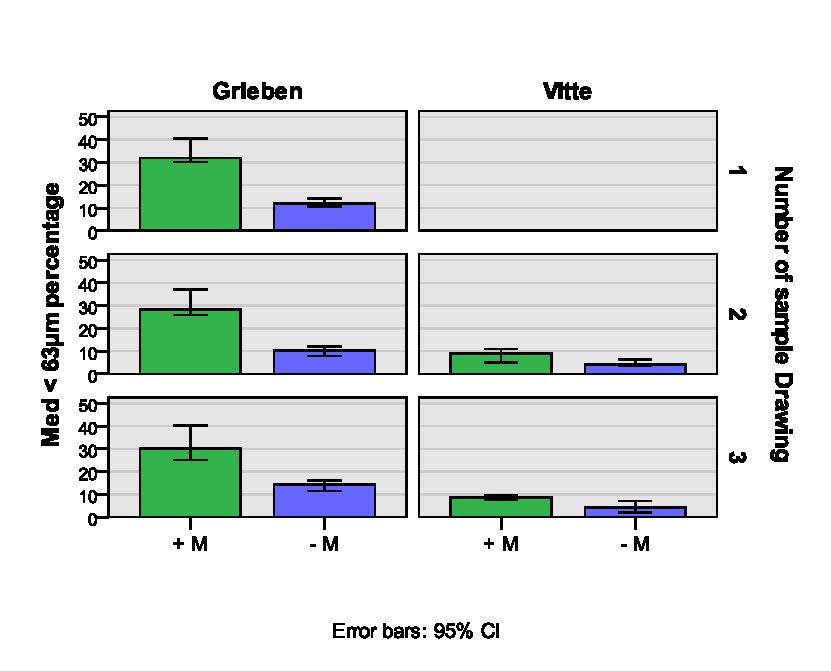
\includegraphics[width=\textwidth]{images/sedimentparameter/S_Parameter_63_neu1.eps}
\end{figure}
\end{column}
\begin{column}{5.5cm}
\pause
Organischer Gehalt
\visible<2>{
\begin{figure}
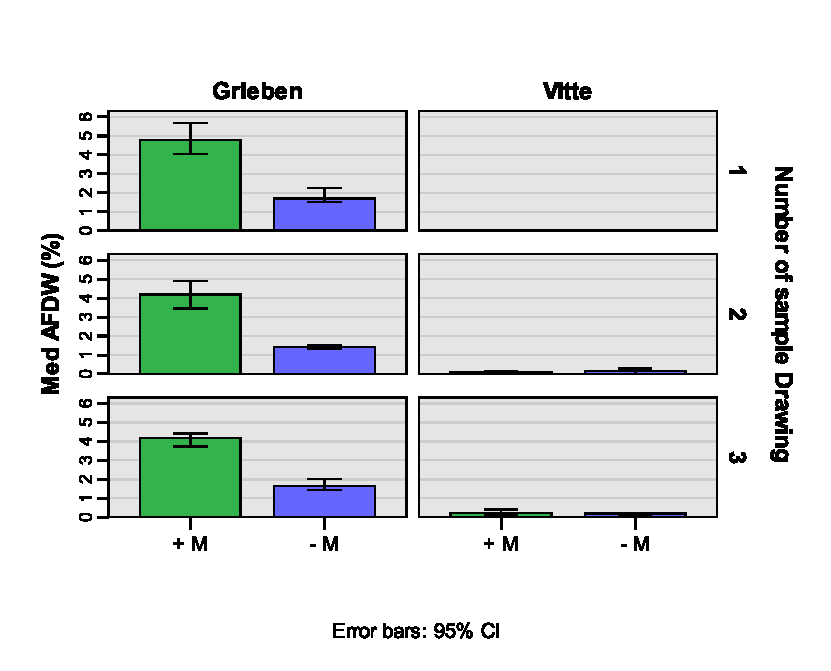
\includegraphics[width=\textwidth]{images/sedimentparameter/afdg_neu1.eps}
\end{figure}}
\end{column}
\end{columns}
\end{frame}

\subsection{Fazit}
\begin{frame}
\begin{enumerate}
\item Fazit1
\item Fazit2
\end{enumerate}
\end{frame}

\section{Quellen}
\begin{frame}
\frametitle{Bildquellen}
\begin{itemize}
\item[1] \textsc{Engelen, Bert}, http://www.pmbio.icbm.de/expeditions/leg301/subproben.jpg 
[Aufruf 8.5.2014; 13:59]
\item[2] \textsc{Melbourne Geofabrics}, http://www.treemax.com.au/content/sieves 

[Aufruf 8.5.2014; 12:18]
\item[3]  \textsc{Stäuber, Kurt}, 

http://wisplants.uwsp.edu/scripts/bigphoto.asp 

[Aufruf 8.5.2014; 14:20]

\end{itemize}

\end{frame}

\end{document}
